\documentclass[12pt,a4paper]{report}
\usepackage[margin=1in]{geometry}
\usepackage{graphicx}
\usepackage{hyperref}
\usepackage{booktabs}
\usepackage{longtable}
\usepackage{array}
\usepackage{xcolor}
\usepackage{listings}
\usepackage{tikz}
\usepackage{amsmath}
\usepackage{float}
\usepackage{caption}
\usepackage{subcaption}
\usepackage{enumitem}
\usepackage{titlesec}
\usepackage{fancyhdr}
\usepackage{mdframed}

\usepackage{tcolorbox}
\tcbuselibrary{skins,breakable}

\usetikzlibrary{shapes,arrows,positioning,fit,calc,decorations.pathmorphing,backgrounds}

\hypersetup{
  colorlinks=true,
  linkcolor=blue!60!black,
  urlcolor=blue!60!black,
  citecolor=blue!60!black
}

\definecolor{codebg}{RGB}{246,247,250}
\definecolor{codefg}{RGB}{30,30,30}
\definecolor{codecomment}{RGB}{106,115,125}
\definecolor{accent}{RGB}{119,89,194}
\definecolor{success}{RGB}{63,185,80}
\definecolor{warning}{RGB}{200,160,0}
\definecolor{danger}{RGB}{200,64,64}
\definecolor{discord}{RGB}{88,101,242}

\lstset{
  backgroundcolor=\color{codebg},
  basicstyle=\ttfamily\footnotesize\color{codefg},
  breaklines=true,
  frame=single,
  rulecolor=\color{gray!30},
  keywordstyle=\bfseries\color{accent},
  commentstyle=\itshape\color{codecomment},
  stringstyle=\color{success!70!black},
  numbers=left,
  numberstyle=\tiny\color{gray!60},
  xleftmargin=2em
}

\pagestyle{fancy}
\fancyhf{}
\fancyhead[L]{\small\textit{Complaint Management System --- SRS \& Design Report}}
\fancyhead[R]{\small\thepage}
\fancyfoot[L]{\small Faculty of Technology, Delhi University \textbullet{} CSE-A}
\fancyfoot[R]{\small Software Engineering}
\renewcommand{\headrulewidth}{0.4pt}
\renewcommand{\footrulewidth}{0.4pt}

\begin{document}

%% ============================================================
%%  TITLE PAGE
%% ============================================================
\begin{titlepage}
\centering

%% ── University logo ──────────────────────────────────────────────────────────

\includegraphics[width=3.5cm]{images/du_logo.png}\\[0.6em]

%% ── Institution block ────────────────────────────────────────────────────────
{\Large\bfseries Faculty of Technology}\\[0.3em]
{\large\bfseries University of Delhi}\\[0.2em]
{\normalsize Department of Computer Science \& Engineering}\\[0.15em]
{\normalsize CSE-A}\\[1.2em]

\rule{\linewidth}{0.8pt}\\[1em]

%% ── Report title ─────────────────────────────────────────────────────────────
{\LARGE\bfseries Complaint Management System}\\[0.5em]
{\large\bfseries Software Requirements Specification\\[0.2em]
\& Extended Design Report}\\[0.8em]

{\normalsize Subject: \textbf{Software Engineering}}\\[1.2em]

\rule{\linewidth}{0.8pt}\\[2em]

%% ── Team members ─────────────────────────────────────────────────────────────
{\large\bfseries Project Team}\\[0.6em]
\begin{tabular}{@{}clc@{}}
\toprule
\textbf{S.No.} & \textbf{Name} & \textbf{Roll Number} \\
\midrule
1 & Mayank Goyal     & 24293916114 \\
2 & Prateek Binjola  & 24293916071 \\
3 & Deepanshu Sharma & 24293916082 \\
4 & Krishan Kumar    & 24293916088 \\
5 & Vansh Sahrawat   & 24293916089 \\
\bottomrule
\end{tabular}\\[2em]

\vfill

\end{titlepage}

\tableofcontents
\newpage

%% ============================================================
%%  1.0  INTRODUCTION
%% ============================================================
\chapter{Introduction}

\section{Purpose}
This document is the Software Requirements Specification (SRS) for the
\textbf{Complaint Management System} (CMS), a multi-platform open-source bug
triage ecosystem.  It describes the functional and non-functional requirements,
system constraints, external interfaces, and extended design artefacts required
to build, deploy, and maintain the system.

The intended audience includes:
\begin{itemize}
  \item Development team members implementing the system.
  \item External examiners evaluating the project submission.
  \item Future maintainers extending the platform.
\end{itemize}

\section{Scope}
The CMS is designed to solve a real-world pain-point articulated by open-source
maintainers: the inability to triage community bug reports efficiently.  Three
core capabilities distinguish it from existing tools:

\begin{enumerate}
  \item \textbf{Discord Buffer Gateway} --- Community complaints arrive via
    Discord Forum Channels, keeping the upstream GitHub issue tracker pristine.
  \item \textbf{Proactive AI Deduplication} --- A vector-embedding pipeline
    detects duplicate reports the moment they are submitted.
  \item \textbf{Decoupled Read-Only Mirror} --- A blazing-fast, login-free
    public frontend lets anyone browse confirmed bugs without an account.
\end{enumerate}

\section{Definitions, Acronyms, and Abbreviations}

\begin{longtable}{>{\bfseries}p{3.5cm} p{10cm}}
\toprule
Term & Definition \\
\midrule
\endhead
CMS & Complaint Management System (this project). \\
SRS & Software Requirements Specification. \\
Discord Gateway & The Discord Forum Channel used as the community intake
                   buffer for incoming bug reports. \\
Triage & The act of reviewing, classifying, and routing incoming issues. \\
Promotion & Moving a validated Discord complaint onto the GitHub issue tracker. \\
Kanban Board & Visual board tracking active issues across workflow stages. \\
AI Similarity & Cosine-similarity score between a new report's vector embedding
                 and existing issues in the knowledge base. \\
ORM & Object-Relational Mapper (Prisma in this project). \\
SSR & Server-Side Rendering (Next.js App Router). \\
RSC & React Server Component. \\
PR & Pull Request on GitHub. \\
CI & Continuous Integration pipeline status. \\
CUID & Collision-resistant Unique Identifier used as  key. \\
\bottomrule
\end{longtable}

\section{Overview}
The remainder of this document is structured as follows:
\begin{itemize}
  \item \textbf{Chapter 2} --- Overall Description: product perspective, user
    classes, assumptions, and constraints.
  \item \textbf{Chapter 3} --- Specific Requirements: functional requirements,
    non-functional requirements, and use cases.
  \item \textbf{Chapter 4} --- Software Design: architecture, class diagrams,
    sequence diagrams, database schema, and security design.
  \item \textbf{Chapter 5} --- Traceability matrix.
  \item \textbf{Chapter 6} --- Code \& repository information.
  \item \textbf{Chapter 7} --- Deployment screenshots.
  \item \textbf{Chapter 8} --- User Manual.
  \item \textbf{Chapter 9} --- Summary.
\end{itemize}

%% ============================================================
%%  2.0  OVERALL DESCRIPTION
%% ============================================================
\chapter{Overall Description}

\section{Product Perspective}
The CMS is a standalone, self-hosted web application that sits between a
community of non-technical users (on Discord) and a software development team
(on GitHub).  Figure~\ref{fig:context-diagram} shows the system context.

\begin{figure}[H]
\centering
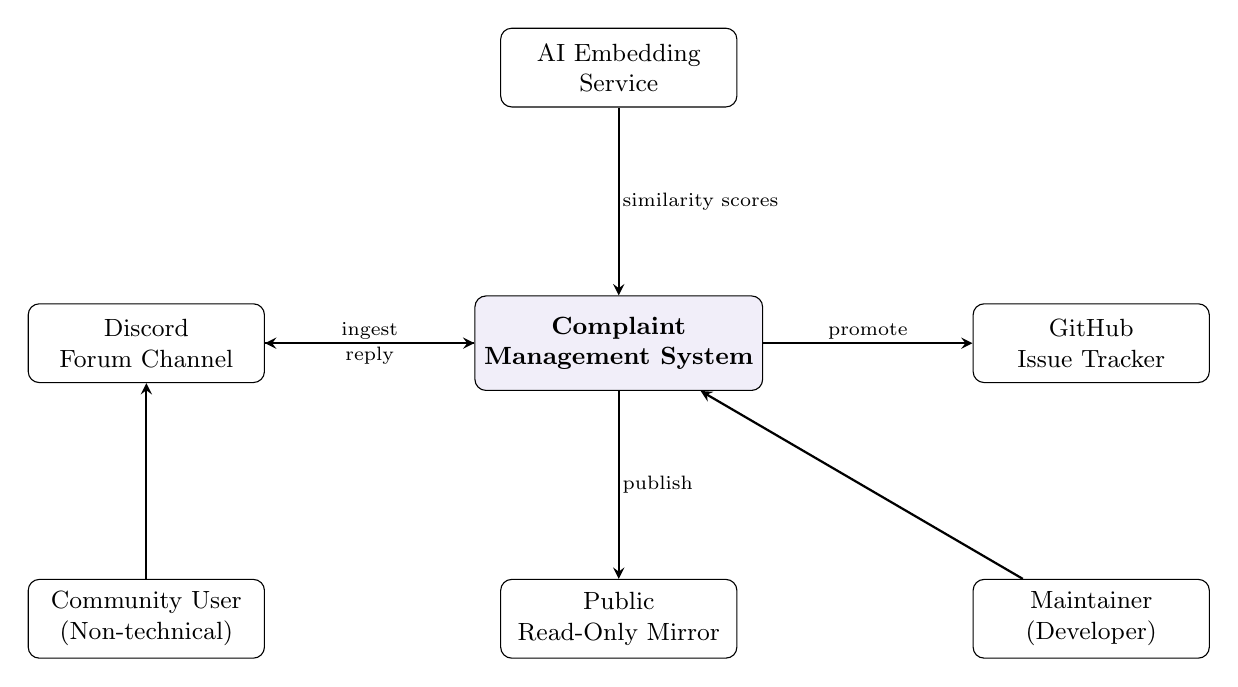
\begin{tikzpicture}[
  box/.style={draw,rounded corners,fill=white,minimum width=3cm,minimum height=1cm,align=center,font=\small},
  sysbox/.style={draw,rounded corners,fill=accent!10,minimum width=3.2cm,minimum height=1.2cm,align=center,font=\small\bfseries},
  arr/.style={->,>=stealth,thick},
  lbl/.style={font=\scriptsize,fill=white,inner sep=1pt}
]
\node[box]    (discord)    at (-6,0)   {Discord\\Forum Channel};
\node[sysbox] (cms)        at (0,0)    {Complaint\\Management System};
\node[box]    (github)     at (6,0)    {GitHub\\Issue Tracker};
\node[box]    (user)       at (-6,-3.5){Community User\\(Non-technical)};
\node[box]    (maintainer) at (6,-3.5) {Maintainer\\(Developer)};
\node[box]    (ai)         at (0,3.5)  {AI Embedding\\Service};
\node[box]    (public)     at (0,-3.5) {Public\\Read-Only Mirror};

% Discord -> CMS (ingest, slightly above midpoint)
\draw[arr] (discord.east) -- (cms.west)
  node[lbl,pos=0.5,above]{ingest};
% CMS -> Discord (reply, slightly below)
\draw[arr] (cms.west) -- (discord.east)
  node[lbl,pos=0.5,below]{reply};
\draw[arr] (cms) -- (github)   node[lbl,midway,above]{promote};
\draw[arr] (user) -- (discord);
\draw[arr] (maintainer) -- (cms);
\draw[arr] (ai)  -- (cms)      node[lbl,midway,right]{similarity scores};
\draw[arr] (cms) -- (public)   node[lbl,midway,right]{publish};
\end{tikzpicture}
\caption{System Context Diagram --- CMS and its external actors}
\label{fig:context-diagram}
\end{figure}

\section{Product Functions}
At the highest level the system provides:
\begin{enumerate}
  \item \textbf{Triage Inbox} --- Displays all Discord-sourced complaints in a
    dense, sortable table with priority, AI similarity score, reporter avatar,
    age, and status.  Supports keyboard-driven navigation (j/k) and one-key
    actions (p = promote, x = spam, e = done).
  \item \textbf{Kanban Board} --- Drag-and-drop board for active (GitHub-source)
    issues across five workflow stages: Backlog, Todo, In Progress, In Review,
    Done.
  \item \textbf{Issue Drawer} --- Animated slide-over panel with full issue
    context, dual-tab chat (Internal Notes / Public Reply), assignee and label
    metadata, linked PRs with CI dots, and context-aware action buttons.
  \item \textbf{AI Deduplication} --- Similarity score stored on each issue;
    visual progress bar and colour-coded alert in both the triage table and
    drawer.
  \item \textbf{Promote Pipeline} --- One-click workflow that creates a GitHub
    issue via REST API, posts a Discord reply with the new issue URL, and moves
    the complaint into the Backlog column.
  \item \textbf{Bulk Actions} --- Multi-select checkbox + bulk-promote and
    bulk-spam for high-volume triage sessions.
  \item \textbf{Command Palette} --- \texttt{Cmd/Ctrl+K} modal with grouped
    navigation and action commands.
  \item \textbf{Create Complaint} --- Modal form to directly create internal
    (GitHub-source) complaints with title, description, and priority.
\end{enumerate}

\section{User Classes and Characteristics}

\begin{longtable}{>{\bfseries}p{3cm} p{4.5cm} p{5.5cm}}
\toprule
User Class & Description & Needs \\
\midrule
\endhead
Maintainer & Core developer with full dashboard access & Fast triage, keyboard shortcuts, action buttons, internal notes \\
Community User & Non-technical end-user on Discord & Zero-friction bug reporting, no account needed \\
Anonymous Browser & Read-only public mirror visitor & Searchable, SEO-indexed bug list without login \\
\bottomrule
\end{longtable}

\section{Operating Environment}
\begin{itemize}
  \item \textbf{Server}: Node.js 20 LTS, Next.js 16 (App Router), running on
    any Linux/macOS host or Docker container.
  \item \textbf{Database}: PostgreSQL 16 (via Docker in development; any
    managed PostgreSQL service in production).
  \item \textbf{ORM}: Prisma 7 with \texttt{@prisma/adapter-pg} driver adapter.
  \item \textbf{Browser}: Modern Chromium/Firefox with JavaScript enabled.
  \item \textbf{External APIs}: Discord Bot API v10, GitHub REST API v2022-11-28.
\end{itemize}

\section{Design and Implementation Constraints}
\begin{itemize}
  \item Must use Next.js App Router exclusively (no Pages Router).
  \item Database schema is managed by Prisma schema file; no raw SQL migrations
    in application code.
  \item GitHub and Discord integrations are optional; the system must degrade
    gracefully when \texttt{GITHUB\_TOKEN} or \texttt{DISCORD\_BOT\_TOKEN} are
    not set.
  \item The public mirror must not require authentication.
  \item Title word limit is enforced at 200 words.
\end{itemize}

\section{Assumptions and Dependencies}
\begin{itemize}
  \item Docker is available on the developer's machine for local PostgreSQL.
  \item The Discord bot has \texttt{Send Messages} and
    \texttt{Read Message History} permissions.
  \item The GitHub Personal Access Token has \texttt{repo} scope.
  \item AI similarity scores are pre-computed and stored; the live embedding
    service is a separate concern outside this MVP scope.
\end{itemize}
%% ============================================================
%%  3.0  SPECIFIC REQUIREMENTS
%% ============================================================
\chapter{Specific Requirements}

\section{External Interface Requirements}

\subsection{User Interfaces}
\begin{itemize}
  \item The web application shall render a responsive, dark-themed dashboard
    (background \texttt{\#1f2023}).
  \item Navigation shall be accessible via both mouse click and keyboard
    shortcut without relying solely on either.
  \item The Triage Inbox shall present data in a scrollable table with sticky
    header row.
  \item The Kanban Board shall support drag-and-drop using pointer and keyboard
    sensors (\texttt{@dnd-kit}).
  \item The Issue Drawer shall animate in from the right with a 200\,ms ease
    transition.
\end{itemize}

\subsection{Hardware Interfaces}
No special hardware is required beyond a standard x86-64 or ARM64 server
capable of running Node.js 20.

\subsection{Software Interfaces}
\begin{longtable}{>{\bfseries}p{3.5cm} p{9cm}}
\toprule
Interface & Description \\
\midrule
\endhead
Discord API v10 & REST endpoint \texttt{POST /channels/\{id\}/messages} used to
  send promotion acknowledgement replies to Discord threads. \\
GitHub API v2022-11-28 & REST endpoint \texttt{POST /repos/\{owner\}/\{repo\}/issues}
  used to create GitHub issues from validated Discord complaints. \\
PostgreSQL 16 & Relational database accessed exclusively through Prisma client;
  connection via \texttt{pg} driver adapter. \\
\bottomrule
\end{longtable}

\subsection{Communication Interfaces}
All external API calls use HTTPS/TLS 1.2+.  Database connections use TCP
within the Docker network or a private cloud VPC.

\section{Functional Requirements}

\subsection{Triage Inbox}

\begin{longtable}{>{\bfseries}p{1.8cm} p{4.5cm} p{6.5cm}}
\toprule
ID & Name & Description \\
\midrule
\endhead
FR-01 & List Discord Issues & System shall display all DISCORD-source issues with
  status \texttt{TRIAGE\_PENDING}, \texttt{TRIAGE\_SPAM}, or
  \texttt{TRIAGE\_PROMOTED} in the inbox. \\
FR-02 & Filter Triage View & Maintainer can filter by: Pending, All, Flagged
  Duplicate, Promoted, Spam using tab selectors. \\
FR-03 & Keyboard Navigation & Pressing \texttt{j}/\texttt{k} shall move the
  focused row cursor down/up; the cursor shall scroll into view. \\
FR-04 & Promote Issue & Pressing \texttt{p}, clicking the promote icon, or using
  the command palette shall invoke \texttt{promoteIssue()}. \\
FR-05 & Mark Spam & Pressing \texttt{x} or clicking the spam icon shall set
  status to \texttt{TRIAGE\_SPAM}. \\
FR-06 & Mark Done & Pressing \texttt{e} shall set status to \texttt{DONE}. \\
FR-07 & Bulk Select & Selecting 2+ rows shall display the Bulk Action Bar. \\
FR-08 & Bulk Promote & Bulk Action Bar ``Promote All'' shall call
  \texttt{bulkPromote()} for each selected issue. \\
FR-09 & Bulk Spam & Bulk Action Bar ``Spam All'' shall call
  \texttt{bulkSpam()} in a single \texttt{updateMany} query. \\
FR-10 & Similarity Display & Each row shall display the AI similarity score as
  a percentage and colour-coded progress bar (green $<30\%$, amber
  $30\text{--}65\%$, red $>65\%$). \\
\bottomrule
\end{longtable}

\subsection{Kanban Board}

\begin{longtable}{>{\bfseries}p{1.8cm} p{4.5cm} p{6.5cm}}
\toprule
ID & Name & Description \\
\midrule
\endhead
FR-11 & Display Board Columns & Board shall render five columns: Backlog, Todo,
  In Progress, In Review, Done, each showing GitHub-source issues. \\
FR-12 & Drag-and-Drop Cards & Maintainer shall drag an issue card between
  columns; the UI updates optimistically and the server is called. \\
FR-13 & Card Metadata & Each card shall show: issue number, title, priority
  dot, label chips, linked PR count with CI status dot, assignee avatars. \\
FR-14 & Milestone Progress & If a milestone exists, the board header shall show
  a progress bar with closed/total count and percentage. \\
FR-15 & Move Status Persist & \texttt{moveKanbanCard()} shall update
  \texttt{Issue.status} and \texttt{lastActivityAt} in the database. \\
\bottomrule
\end{longtable}

\subsection{Issue Drawer}

\begin{longtable}{>{\bfseries}p{1.8cm} p{4.5cm} p{6.5cm}}
\toprule
ID & Name & Description \\
\midrule
\endhead
FR-16 & Fetch Issue Detail & Opening the drawer shall call
  \texttt{GET /api/issues/\{id\}} and render full issue data. \\
FR-17 & Discord Thread View & For DISCORD-source issues, the drawer shall
  render the original message and all replies in a thread-style layout. \\
FR-18 & AI Similarity Block & When \texttt{similarityScore > 0.1}, the drawer
  shall display a colour-coded similarity card with merge/dismiss actions. \\
FR-19 & Dual Chat Tabs & Drawer shall provide ``Internal Notes'' (private) and
  ``Public Reply'' (syncs to Discord) tabs. \\
FR-20 & Focus Mode & Pressing \texttt{f} or the expand icon shall toggle the
  drawer to full-width (\texttt{90vw}). \\
FR-21 & Promote from Drawer & Footer ``Promote to GitHub'' button shall invoke
  \texttt{promoteIssue()} and close the drawer. \\
FR-22 & Copy Link & Clicking the copy icon shall write the current URL to
  clipboard via \texttt{navigator.clipboard}. \\
FR-23 & Metadata Sidebar & Right panel shall show assignees, labels, milestone,
  GitHub issue number, and linked PRs with CI status. \\
\bottomrule
\end{longtable}

\subsection{Promote Pipeline}

\begin{longtable}{>{\bfseries}p{1.8cm} p{4.5cm} p{6.5cm}}
\toprule
ID & Name & Description \\
\midrule
\endhead
FR-24 & Create GitHub Issue & When GitHub integration is enabled,
  \texttt{promoteIssue()} shall call GitHub REST API to create a new issue with
  title, formatted body, and labels. \\
FR-25 & Discord Notification & When Discord integration is enabled and the
  issue has a \texttt{discordThreadId}, the system shall post a promotion
  comment back to the Discord thread. \\
FR-26 & Label Retry & If GitHub returns 422 (labels not found), the system
  shall retry without labels. \\
FR-27 & Status Update & Promoted issue shall have \texttt{source} set to
  \texttt{GITHUB} and \texttt{status} set to \texttt{BACKLOG}. \\
\bottomrule
\end{longtable}

\subsection{Create Complaint}

\begin{longtable}{>{\bfseries}p{1.8cm} p{4.5cm} p{6.5cm}}
\toprule
ID & Name & Description \\
\midrule
\endhead
FR-28 & Open Create Modal & Pressing \texttt{c} or clicking ``New Complaint''
  in the top bar shall open the create modal. \\
FR-29 & Validate Title & Title must not exceed 200 words; violation shall throw
  a descriptive error. \\
FR-30 & Persist Complaint & Submitting the form shall invoke
  \texttt{createIssue()} which creates an issue with
  \texttt{source=GITHUB}, \texttt{status=TODO}, and auto-increments the
  per-organisation issue number. \\
FR-31 & Post-Create Navigation & After successful creation, the app shall
  navigate to the Active Board. \\
\bottomrule
\end{longtable}

\subsection{Command Palette and Keyboard Shortcuts}

\begin{longtable}{>{\bfseries}p{1.8cm} p{4.5cm} p{6.5cm}}
\toprule
ID & Name & Description \\
\midrule
\endhead
FR-32 & Open Palette & \texttt{Ctrl/Cmd+K} shall open the command palette
  powered by \texttt{cmdk}. \\
FR-33 & Navigate Commands & Palette groups: Navigate (triage, board, settings),
  Actions (promote, spam, done, merge, flag), View (focus mode). \\
FR-34 & Go-to Sequences & \texttt{g→t} (triage), \texttt{g→b} (board),
  \texttt{g→s} (settings) shall navigate via
  \texttt{tinykeys} two-key sequences. \\
\bottomrule
\end{longtable}

\section{Non-Functional Requirements}

\begin{longtable}{>{\bfseries}p{2cm} p{4cm} p{7cm}}
\toprule
ID & Category & Requirement \\
\midrule
\endhead
NFR-01 & Performance & Triage page initial server response shall complete within
  500\,ms on a local machine with $\leq$\,1000 issues. \\
NFR-02 & Security & All maintainer actions (promote, spam, create) shall
  execute as Next.js Server Actions; no sensitive logic runs client-side. \\
NFR-03 & Security & API tokens (\texttt{GITHUB\_TOKEN},
  \texttt{DISCORD\_BOT\_TOKEN}) shall never be exposed to the browser; they
  shall only be read from environment variables on the server. \\
NFR-04 & Reliability & Drag-and-drop moves shall employ optimistic UI with
  automatic rollback on server failure. \\
NFR-05 & Usability & All primary triage actions shall be completable without
  lifting hands from the keyboard. \\
NFR-06 & Scalability & Database queries for the board and triage shall include
  only necessary joins via Prisma \texttt{include}, avoiding N+1 queries. \\
NFR-07 & Maintainability & TypeScript strict mode shall be enabled; all server
  action function signatures shall be explicitly typed. \\
NFR-08 & Accessibility & Interactive elements shall have \texttt{aria-label}
  attributes; keyboard focus shall be visible. \\
NFR-09 & Deployability & A single \texttt{npm run setup} command shall
  bootstrap the full local development environment. \\
NFR-10 & Data Integrity & \texttt{IssueAssignee} and \texttt{IssueLabel} join
  tables shall cascade-delete on parent \texttt{Issue} deletion. \\
\bottomrule
\end{longtable}

\section{Use Cases}

\subsection{UC-01: Triage a Discord Complaint}
\begin{tcolorbox}[colback=gray!5,colframe=accent,title=UC-01 --- Triage Discord Complaint]
\textbf{Actors:} Maintainer \\
\textbf{Preconditions:} Maintainer is on \texttt{/dashboard/triage}; at least one DISCORD-source complaint with status \texttt{TRIAGE\_PENDING} exists. \\
\textbf{Main Flow:}
\begin{enumerate}
  \item Maintainer presses \texttt{j} to move cursor to first pending complaint.
  \item System highlights the row and scrolls it into view.
  \item Maintainer presses \texttt{Enter} to open the Issue Drawer.
  \item Drawer slides in; system fetches full issue data from \texttt{/api/issues/\{id\}}.
  \item Maintainer reviews the Discord thread context and AI similarity score.
  \item Maintainer presses \texttt{p} (or clicks ``Promote to GitHub'' in drawer).
  \item System calls \texttt{promoteIssue()}: creates GitHub issue, posts Discord reply, updates DB.
  \item Toast notification confirms promotion; drawer closes; triage list refreshes.
\end{enumerate}
\textbf{Alternate Flow A (Spam):} At step 6, maintainer presses \texttt{x}; issue is marked \texttt{TRIAGE\_SPAM}. \\
\textbf{Postconditions:} Issue has \texttt{source=GITHUB}, \texttt{status=BACKLOG}, appears on Kanban board.
\end{tcolorbox}

\subsection{UC-02: Move Issue on Kanban Board}
\begin{tcolorbox}[colback=gray!5,colframe=accent,title=UC-02 --- Move Kanban Card]
\textbf{Actors:} Maintainer \\
\textbf{Preconditions:} At least one issue exists in the \texttt{BACKLOG} or \texttt{TODO} column. \\
\textbf{Main Flow:}
\begin{enumerate}
  \item Maintainer drags an issue card from \textbf{Todo} to \textbf{In Progress}.
  \item UI optimistically moves the card.
  \item System calls \texttt{moveKanbanCard(issueId, ``IN\_PROGRESS'')}.
  \item Database updates \texttt{Issue.status} and \texttt{lastActivityAt}.
  \item Toast confirms move.
\end{enumerate}
\textbf{Alternate Flow A (Failure):} Server action throws; UI rolls back card to original column; error toast shown. \\
\textbf{Postconditions:} Issue status is \texttt{IN\_PROGRESS} in database.
\end{tcolorbox}

\subsection{UC-03: Bulk Spam Session}
\begin{tcolorbox}[colback=gray!5,colframe=accent,title=UC-03 --- Bulk Spam]
\textbf{Actors:} Maintainer \\
\textbf{Main Flow:}
\begin{enumerate}
  \item Maintainer selects multiple rows using checkboxes.
  \item Bulk Action Bar appears at the bottom of the screen.
  \item Maintainer clicks ``Spam All''.
  \item System calls \texttt{bulkSpam(selectedIds)}.
  \item All selected issues updated to \texttt{TRIAGE\_SPAM} in a single \texttt{updateMany}.
  \item Selection clears; triage view refreshes.
\end{enumerate}
\textbf{Postconditions:} All selected issues have \texttt{status=TRIAGE\_SPAM}.
\end{tcolorbox}

\subsection{UC-04: Create Internal Complaint}
\begin{tcolorbox}[colback=gray!5,colframe=accent,title=UC-04 --- Create Complaint]
\textbf{Actors:} Maintainer \\
\textbf{Main Flow:}
\begin{enumerate}
  \item Maintainer presses \texttt{c} to open the Create Complaint modal.
  \item Fills in title, description, and priority.
  \item Presses \texttt{Ctrl+Enter} or clicks ``Create Complaint''.
  \item System validates title $\leq$ 200 words.
  \item \texttt{createIssue()} creates DB record with \texttt{source=GITHUB}, \texttt{status=TODO}.
  \item App navigates to Active Board; new card appears in Todo column.
\end{enumerate}
\textbf{Postconditions:} New issue persisted with auto-incremented per-org number.
\end{tcolorbox}

\subsection{UC-05: View AI Duplicate Alert}
\begin{tcolorbox}[colback=gray!5,colframe=accent,title=UC-05 --- AI Duplicate Detection]
\textbf{Actors:} Maintainer (triggered automatically on issue ingest) \\
\textbf{Main Flow:}
\begin{enumerate}
  \item Maintainer opens the Issue Drawer for a complaint with
    \texttt{similarityScore > 0.1}.
  \item Drawer renders the AI Similarity section with progress bar and
    percentage badge.
  \item If \texttt{duplicateOfId} is set, the UI shows ``Possible duplicate of
    \#N'' with Merge and Dismiss buttons.
  \item Maintainer clicks ``Merge into \#N'' (phase-2 placeholder in current
    build; toast shown).
\end{enumerate}
\textbf{Postconditions:} (Phase 2) Issue marked \texttt{CLOSED} with
\texttt{duplicateOfId} set.
\end{tcolorbox}
%% ============================================================
%%  4.0  SOFTWARE DESIGN
%% ============================================================
\chapter{Software Design}

\section{System Architecture}

The CMS follows a \textbf{Server-Centric Layered Architecture} enabled by the
Next.js 16 App Router.  Figure~\ref{fig:arch} illustrates the four principal
layers.

\begin{figure}[H]
\centering
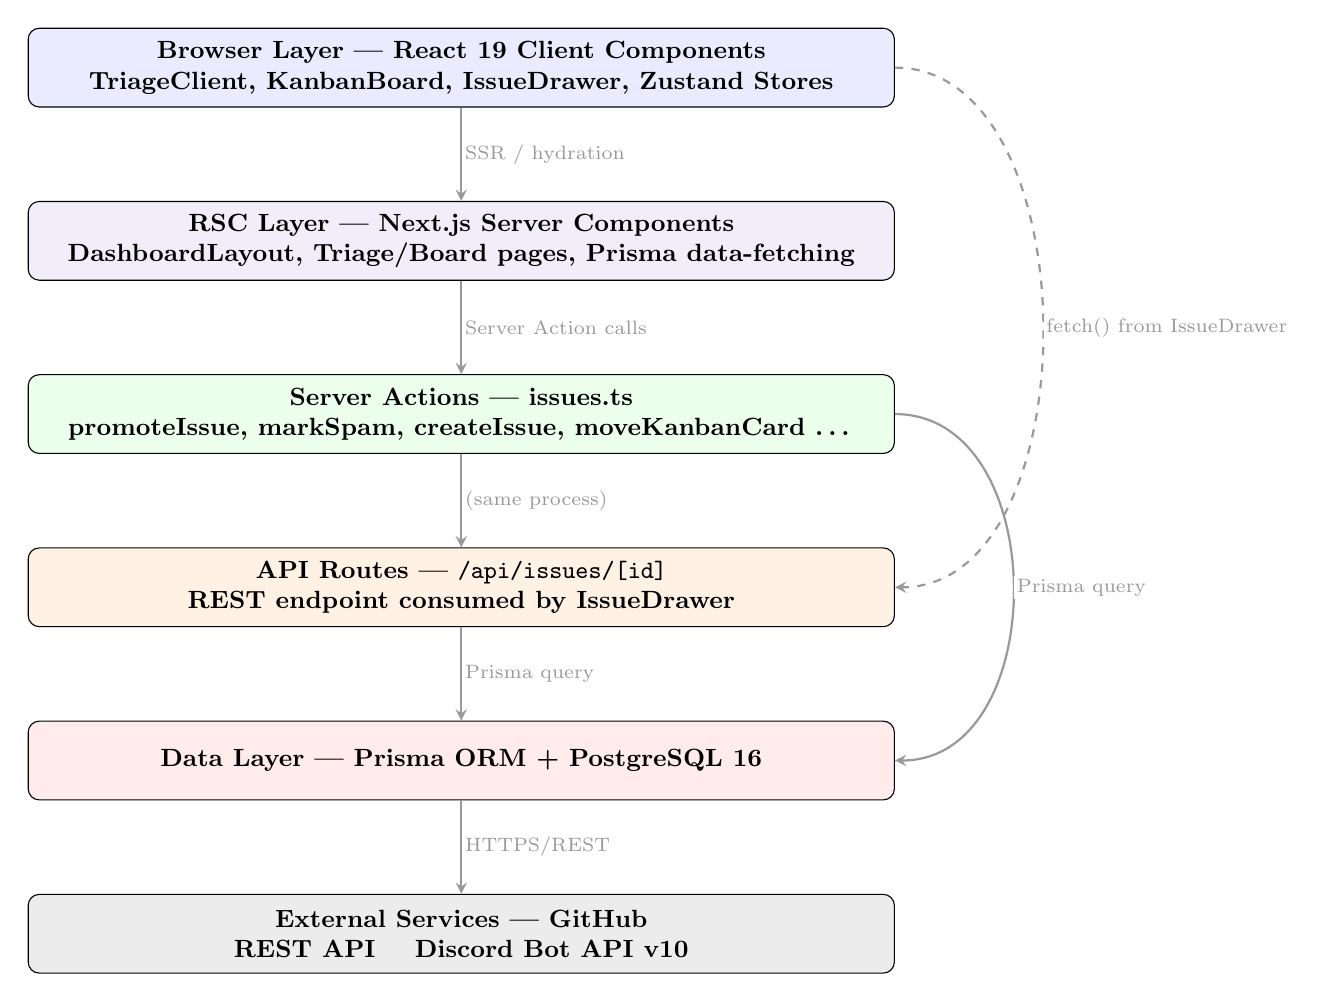
\begin{tikzpicture}[
  lyr/.style={draw,rounded corners,minimum width=11cm,minimum height=1cm,
              align=center,font=\small\bfseries,text width=10.5cm},
  arr/.style={->,>=stealth,thick,gray!80},
  lbl/.style={font=\scriptsize,fill=white,inner sep=1pt}
]
% Stack nodes vertically, centered at x=0
\node[lyr,fill=blue!8]    (browser) at (0, 0)    {Browser Layer --- React 19 Client Components\\TriageClient, KanbanBoard, IssueDrawer, Zustand Stores};
\node[lyr,fill=accent!10] (rsc)     at (0,-2.2)  {RSC Layer --- Next.js Server Components\\DashboardLayout, Triage/Board pages, Prisma data-fetching};
\node[lyr,fill=green!8]   (actions) at (0,-4.4)  {Server Actions --- issues.ts\\promoteIssue, markSpam, createIssue, moveKanbanCard \ldots};
\node[lyr,fill=orange!10] (api)     at (0,-6.6)  {API Routes --- \texttt{/api/issues/[id]}\\REST endpoint consumed by IssueDrawer};
\node[lyr,fill=red!8]     (db)      at (0,-8.8)  {Data Layer --- Prisma ORM + PostgreSQL 16};
\node[lyr,fill=gray!15]   (ext)     at (0,-11.0) {External Services --- GitHub REST API \quad Discord Bot API v10};

% Central downward arrows
\draw[arr] (browser.south) -- (rsc.north)     node[lbl,midway,right]{SSR / hydration};
\draw[arr] (rsc.south)     -- (actions.north) node[lbl,midway,right]{Server Action calls};
\draw[arr] (actions.south) -- (api.north)     node[lbl,midway,right]{(same process)};
\draw[arr] (api.south)     -- (db.north)      node[lbl,midway,right]{Prisma query};
\draw[arr] (actions.east)  .. controls +(2,0) and +(2,0) ..
           (db.east)        node[lbl,pos=0.5,right]{Prisma query};
\draw[arr] (db.south)      -- (ext.north)     node[lbl,midway,right]{HTTPS/REST};

% fetch() side note (client -> api)
\draw[arr,dashed] (browser.east) .. controls +(2.5,0) and +(2.5,0) ..
                  (api.east)      node[lbl,pos=0.5,right]{fetch() from IssueDrawer};
\end{tikzpicture}
\caption{CMS Layered System Architecture}
\label{fig:arch}
\end{figure}

\subsection{Technology Stack Summary}

\begin{longtable}{>{\bfseries}p{3.5cm} p{9cm}}
\toprule
Technology & Role \\
\midrule
\endhead
Next.js 16 (App Router) & Full-stack React framework; RSCs for data fetch, Server Actions for mutations. \\
React 19 & UI component library. \\
TypeScript 5 & Static typing across the entire codebase. \\
Prisma 7 & Type-safe ORM; schema migrations via \texttt{prisma db push}. \\
PostgreSQL 16 & Primary relational database. \\
Zustand 5 & Lightweight client-side state management (drawer, bulk-select, triage cursor). \\
@dnd-kit & Accessible drag-and-drop for Kanban board. \\
Framer Motion 12 & Drawer animation (\texttt{AnimatePresence}, spring transitions). \\
TanStack Query 5 & Optional server-state caching layer. \\
Tiptap 3 & Rich-text editor for note/reply composer. \\
cmdk & Headless command palette. \\
tinykeys 3 & Keyboard shortcut binding (including two-key sequences). \\
Tailwind CSS 4 & Utility-first styling. \\
Sonner 2 & Toast notification system. \\
lucide-react & Icon set. \\
\bottomrule
\end{longtable}

\subsection{Data Flow: Discord Complaint Ingest}

\begin{figure}[H]
\centering
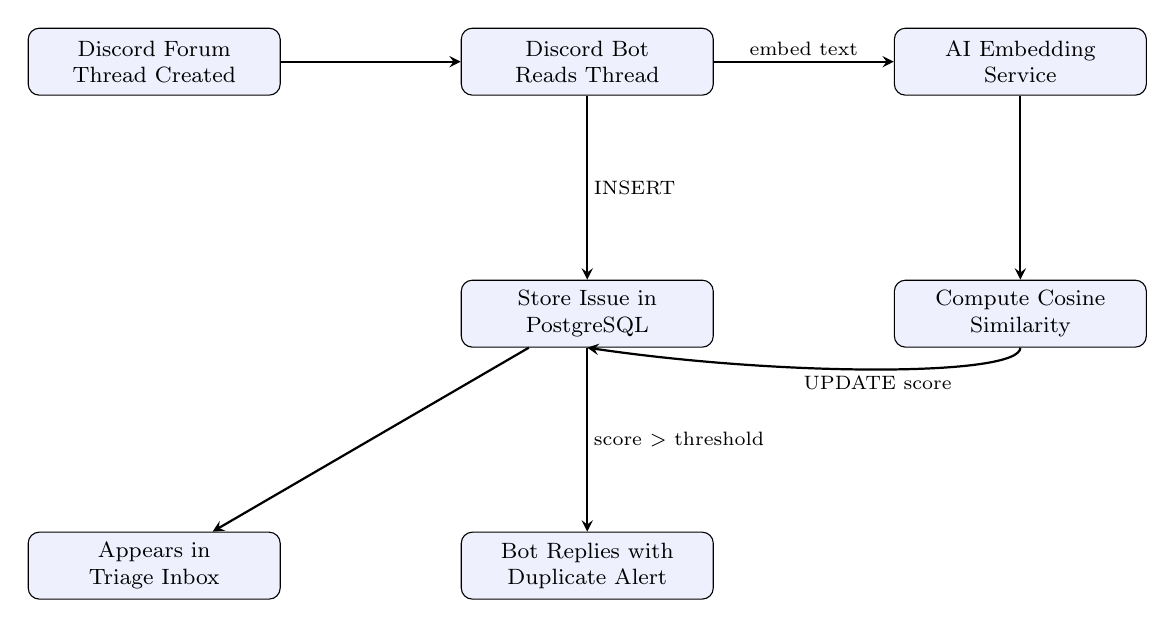
\begin{tikzpicture}[
  proc/.style={draw,rounded corners,fill=discord!10,minimum width=3.2cm,
               minimum height=0.85cm,align=center,font=\footnotesize},
  arr/.style={->,>=stealth,thick},
  lbl/.style={font=\scriptsize,fill=white,inner sep=2pt}
]
% Row 1: three horizontally-spaced nodes
\node[proc] (d)   at (0, 0)    {Discord Forum\\Thread Created};
\node[proc] (b)   at (5.5, 0)  {Discord Bot\\Reads Thread};
\node[proc] (e)   at (11, 0)   {AI Embedding\\Service};
% Row 2: db1 under b, sim under e  – extra vertical gap
\node[proc] (db1) at (5.5,-3.2){Store Issue in\\PostgreSQL};
\node[proc] (sim) at (11,-3.2) {Compute Cosine\\Similarity};
% Row 3
\node[proc] (r)   at (5.5,-6.4){Bot Replies with\\Duplicate Alert};
\node[proc] (ti)  at (0,-6.4)  {Appears in\\Triage Inbox};

\draw[arr] (d)  -- (b);
\draw[arr] (b)  -- (e)    node[lbl,midway,above]{embed text};
\draw[arr] (e)  -- (sim);
\draw[arr] (b)  -- (db1)  node[lbl,midway,right]{INSERT};
% UPDATE score: route the arrow below both nodes to avoid overlap
\draw[arr] (sim.south) .. controls (11,-4.0) and (8,-4.0) .. (db1.south)
  node[lbl,pos=0.5,below]{UPDATE score};
\draw[arr] (db1) -- (r)   node[lbl,midway,right]{score $>$ threshold};
\draw[arr] (db1) -- (ti);
\end{tikzpicture}
\caption{Discord Complaint Ingest and AI Deduplication Data Flow}
\label{fig:ingest-flow}
\end{figure}

\section{Detailed Design}

\subsection{Class Diagrams}

\subsubsection{Domain Model --- Core Entities}

\begin{figure}[H]
\centering
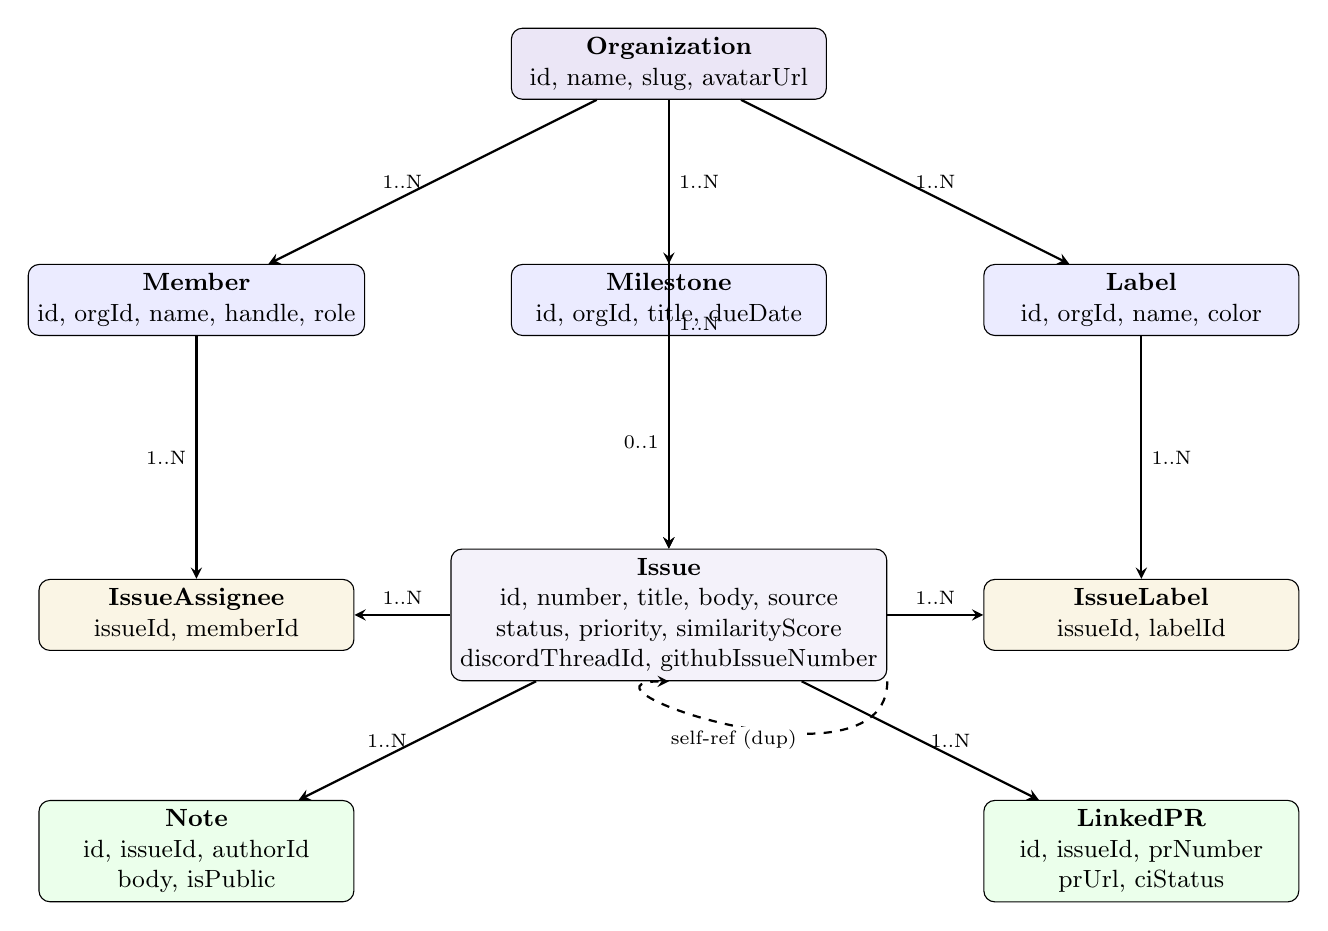
\begin{tikzpicture}[
  cls/.style={draw,fill=blue!6,rounded corners,minimum width=4cm,minimum height=0.8cm,align=center,font=\small},
  arr/.style={->,>=stealth,thick},
  comp/.style={->,>=diamond,thick}
]
% Classes
\node[cls,fill=accent!15] (org)      at (0,6)    {\textbf{Organization}\\id, name, slug, avatarUrl};
\node[cls,fill=blue!8]    (member)   at (-6,3)   {\textbf{Member}\\id, orgId, name, handle, role};
\node[cls,fill=blue!8]    (label)    at (6,3)    {\textbf{Label}\\id, orgId, name, color};
\node[cls,fill=blue!8]    (ms)       at (0,3)    {\textbf{Milestone}\\id, orgId, title, dueDate};
\node[cls,fill=accent!8]  (issue)    at (0,-1)   {\textbf{Issue}\\id, number, title, body, source\\status, priority, similarityScore\\discordThreadId, githubIssueNumber};
\node[cls,fill=green!8]   (note)     at (-6,-4)  {\textbf{Note}\\id, issueId, authorId\\body, isPublic};
\node[cls,fill=green!8]   (pr)       at (6,-4)   {\textbf{LinkedPR}\\id, issueId, prNumber\\prUrl, ciStatus};
\node[cls,fill=warning!10](ia)       at (-6,-1)  {\textbf{IssueAssignee}\\issueId, memberId};
\node[cls,fill=warning!10](il)       at (6,-1)   {\textbf{IssueLabel}\\issueId, labelId};

% Relationships
\draw[arr] (org) -- (member)  node[midway,left,font=\scriptsize]{1..N};
\draw[arr] (org) -- (label)   node[midway,right,font=\scriptsize]{1..N};
\draw[arr] (org) -- (ms)      node[midway,right,font=\scriptsize]{1..N};
\draw[arr] (org) -- (issue)   node[midway,right,font=\scriptsize]{1..N};
\draw[arr] (issue) -- (note)  node[midway,left,font=\scriptsize]{1..N};
\draw[arr] (issue) -- (pr)    node[midway,right,font=\scriptsize]{1..N};
\draw[arr] (issue) -- (ia)    node[midway,above,sloped,font=\scriptsize]{1..N};
\draw[arr] (issue) -- (il)    node[midway,above,sloped,font=\scriptsize]{1..N};
\draw[arr] (member) -- (ia)   node[midway,left,font=\scriptsize]{1..N};
\draw[arr] (label) -- (il)    node[midway,right,font=\scriptsize]{1..N};
\draw[arr] (ms) -- (issue)    node[midway,left,font=\scriptsize]{0..1};
\draw[arr,dashed] (issue.south east) .. controls +(0,-1.5) and +(-1.5,0) .. (issue.south)
  node[pos=0.5,below,font=\scriptsize,fill=white,inner sep=1pt]{self-ref (dup)};
\end{tikzpicture}
\caption{Domain Model Class Diagram (D-CL-01)}
\label{fig:domain-class}
\end{figure}

\subsubsection{Component Architecture Class Diagram}

\begin{figure}[H]
\centering
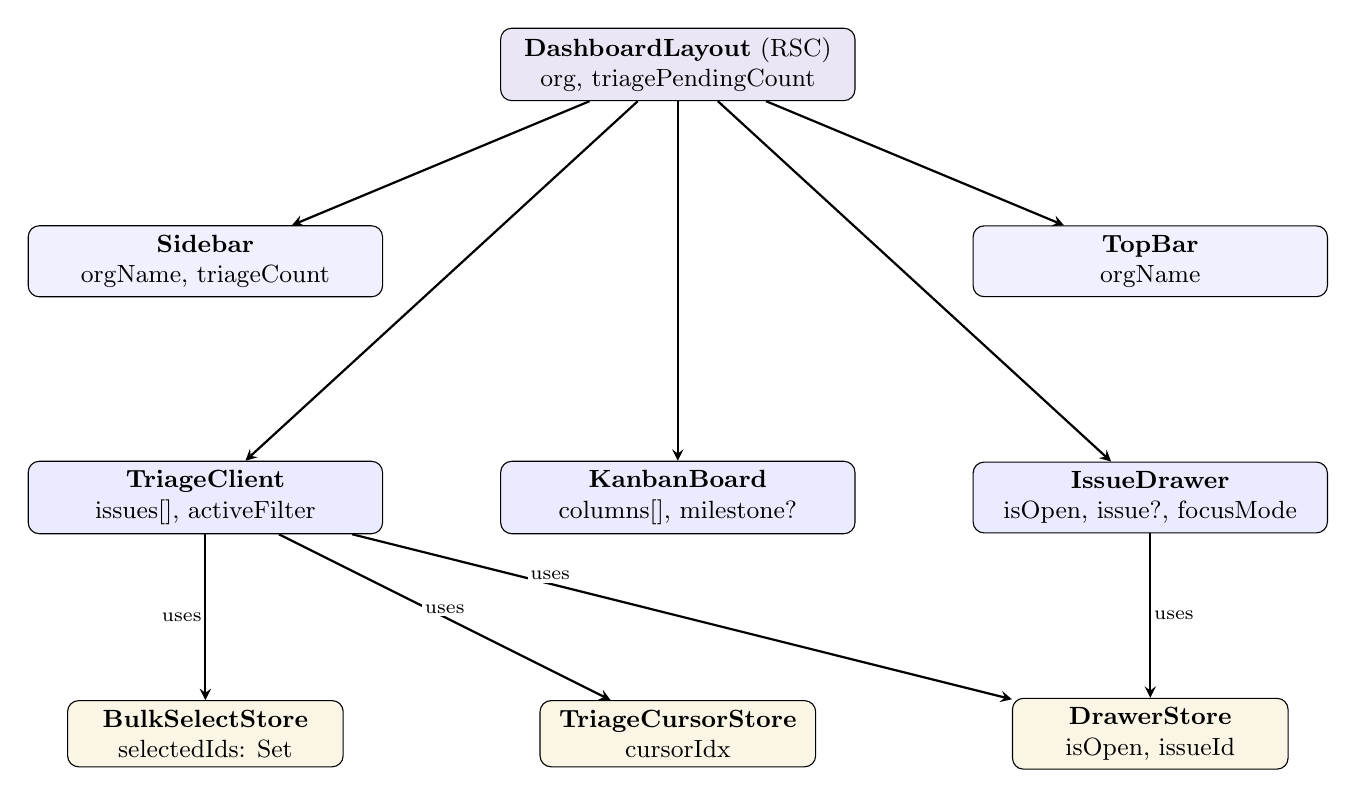
\begin{tikzpicture}[
  cls/.style={draw,fill=blue!6,rounded corners,minimum width=4.5cm,minimum height=0.7cm,align=center,font=\small},
  store/.style={draw,fill=warning!10,rounded corners,minimum width=3.5cm,minimum height=0.7cm,align=center,font=\small},
  arr/.style={->,>=stealth,thick,font=\scriptsize}
]
% RSC / Layout
\node[cls,fill=accent!15] (dl)  at (0,7)    {\textbf{DashboardLayout} (RSC)\\org, triagePendingCount};
\node[cls]                (sb)  at (-6,4.5) {\textbf{Sidebar}\\orgName, triageCount};
\node[cls]                (tb)  at (6,4.5)  {\textbf{TopBar}\\orgName};
% Client components
\node[cls,fill=blue!8]    (tc)  at (-6,1.5) {\textbf{TriageClient}\\issues[], activeFilter};
\node[cls,fill=blue!8]    (kb)  at (0,1.5)  {\textbf{KanbanBoard}\\columns[], milestone?};
\node[cls,fill=blue!8]    (id)  at (6,1.5)  {\textbf{IssueDrawer}\\isOpen, issue?, focusMode};
% Stores
\node[store] (ds)  at (6,-1.5)  {\textbf{DrawerStore}\\isOpen, issueId};
\node[store] (bs)  at (-6,-1.5) {\textbf{BulkSelectStore}\\selectedIds: Set};
\node[store] (tcs) at (0,-1.5)  {\textbf{TriageCursorStore}\\cursorIdx};

% Arrows
\draw[arr] (dl) -- (sb);
\draw[arr] (dl) -- (tb);
\draw[arr] (dl) -- (id);
\draw[arr] (dl) -- (tc);
\draw[arr] (dl) -- (kb);
\draw[arr] (id)  -- (ds)  node[midway,right,font=\scriptsize,fill=white,inner sep=1pt]{uses};
\draw[arr] (tc)  -- (ds)  node[pos=0.3,above,font=\scriptsize,fill=white,inner sep=1pt]{uses};
\draw[arr] (tc)  -- (bs)  node[midway,left,font=\scriptsize,fill=white,inner sep=1pt]{uses};
\draw[arr] (tc)  -- (tcs) node[midway,above,font=\scriptsize,fill=white,inner sep=1pt]{uses};
\end{tikzpicture}
\caption{Component Architecture Class Diagram (D-CL-02)}
\label{fig:component-class}
\end{figure}

\subsection{Sequence Diagrams}

\subsubsection{SD-01: Promote Discord Issue to GitHub}

\begin{figure}[H]
\centering
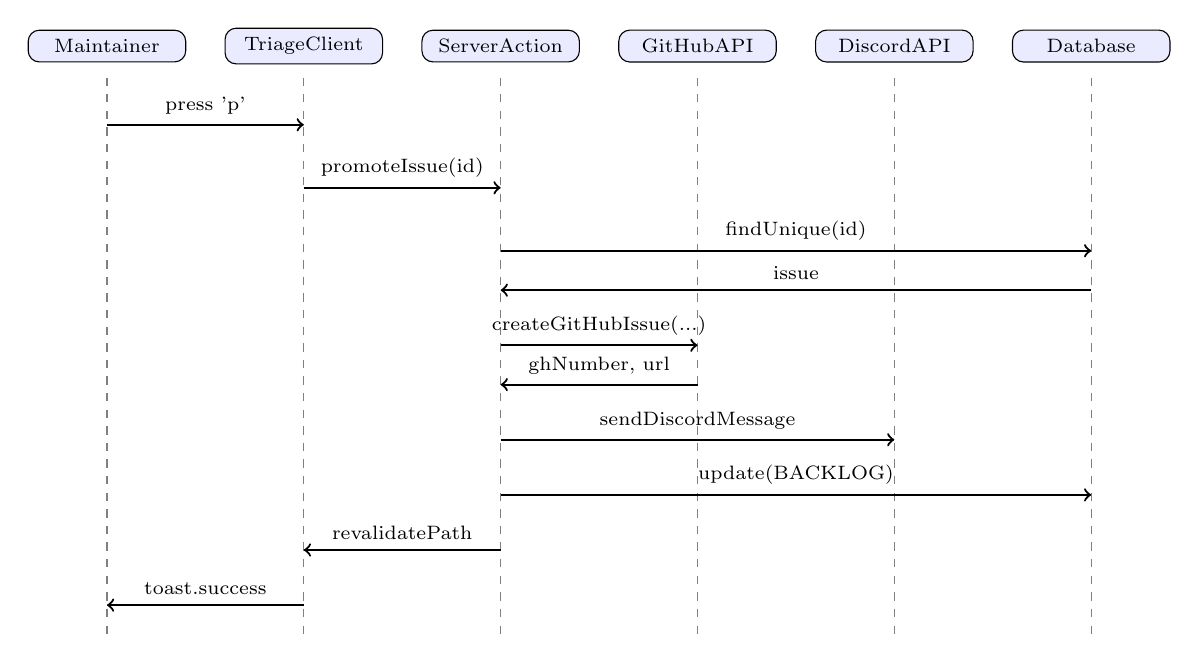
\begin{tikzpicture}[font=\small]
  \def\actors{{"Maintainer","TriageClient","ServerAction","GitHubAPI","DiscordAPI","Database"}}
  % Lifelines
  \foreach \x/\name in {0/Maintainer,2.5/TriageClient,5/ServerAction,7.5/GitHubAPI,10/DiscordAPI,12.5/Database}{
    \node[draw,fill=blue!8,rounded corners,minimum width=2cm,align=center,font=\scriptsize] at (\x,0) {\name};
    \draw[dashed,gray] (\x,-0.4) -- (\x,-7.5);
  }
  % Messages
  \draw[->,thick] (0,-1) -- (2.5,-1) node[midway,above,font=\scriptsize]{press 'p'};
  \draw[->,thick] (2.5,-1.8) -- (5,-1.8) node[midway,above,font=\scriptsize]{promoteIssue(id)};
  \draw[->,thick] (5,-2.6) -- (12.5,-2.6) node[midway,above,font=\scriptsize]{findUnique(id)};
  \draw[<-,thick] (5,-3.1) -- (12.5,-3.1) node[midway,above,font=\scriptsize]{issue};
  \draw[->,thick] (5,-3.8) -- (7.5,-3.8) node[midway,above,font=\scriptsize]{createGitHubIssue(...)};
  \draw[<-,thick] (5,-4.3) -- (7.5,-4.3) node[midway,above,font=\scriptsize]{ghNumber, url};
  \draw[->,thick] (5,-5) -- (10,-5) node[midway,above,font=\scriptsize]{sendDiscordMessage};
  \draw[->,thick] (5,-5.7) -- (12.5,-5.7) node[midway,above,font=\scriptsize]{update(BACKLOG)};
  \draw[->,thick] (5,-6.4) -- (2.5,-6.4) node[midway,above,font=\scriptsize]{revalidatePath};
  \draw[->,thick] (2.5,-7.1) -- (0,-7.1) node[midway,above,font=\scriptsize]{toast.success};
\end{tikzpicture}
\caption{Sequence Diagram: Promote Issue (D-SQ-01)}
\label{fig:sd-promote}
\end{figure}

\subsubsection{SD-02: Kanban Drag-and-Drop}

\begin{figure}[H]
\centering
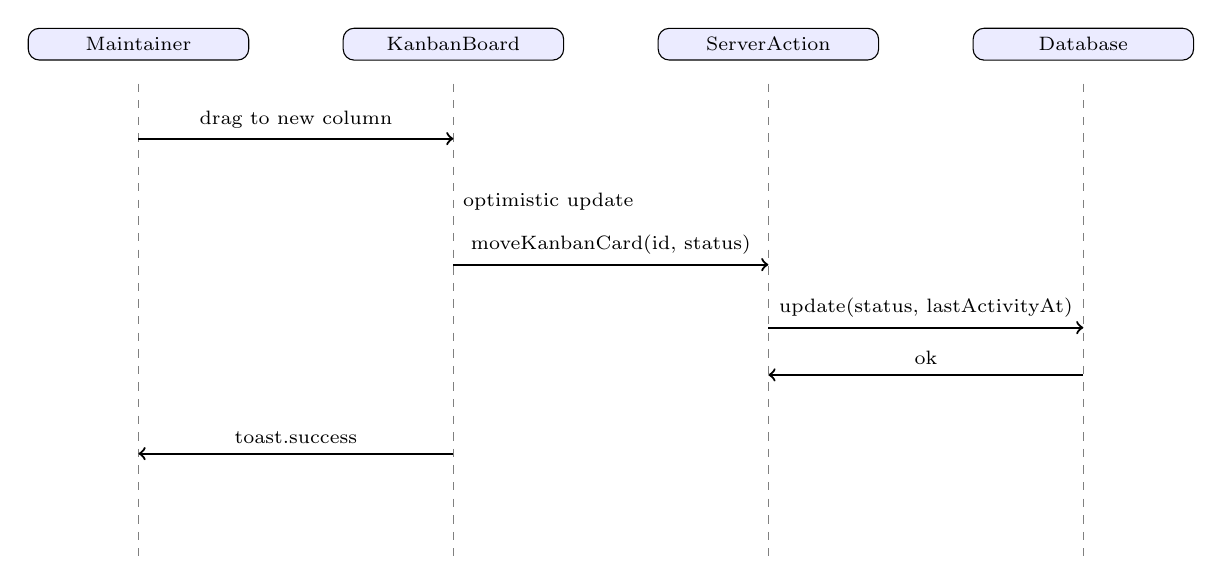
\begin{tikzpicture}[font=\small]
  \foreach \x/\name in {0/Maintainer,4/KanbanBoard,8/ServerAction,12/Database}{
    \node[draw,fill=blue!8,rounded corners,minimum width=2.8cm,align=center,font=\scriptsize] at (\x,0) {\name};
    \draw[dashed,gray] (\x,-0.5) -- (\x,-6.5);
  }
  \draw[->,thick] (0,-1.2) -- (4,-1.2)  node[midway,above,font=\scriptsize]{drag to new column};
  \node[font=\scriptsize,right] at (4,-2.0) {optimistic update};
  \draw[->,thick] (4,-2.8) -- (8,-2.8)  node[midway,above,font=\scriptsize]{moveKanbanCard(id, status)};
  \draw[->,thick] (8,-3.6) -- (12,-3.6) node[midway,above,font=\scriptsize]{update(status, lastActivityAt)};
  \draw[<-,thick] (8,-4.2) -- (12,-4.2) node[midway,above,font=\scriptsize]{ok};
  \draw[->,thick] (4,-5.2) -- (0,-5.2)  node[midway,above,font=\scriptsize]{toast.success};
\end{tikzpicture}
\caption{Sequence Diagram: Kanban Move (D-SQ-02)}
\label{fig:sd-kanban}
\end{figure}

\subsubsection{SD-03: Open Issue Drawer}

\begin{figure}[H]
\centering
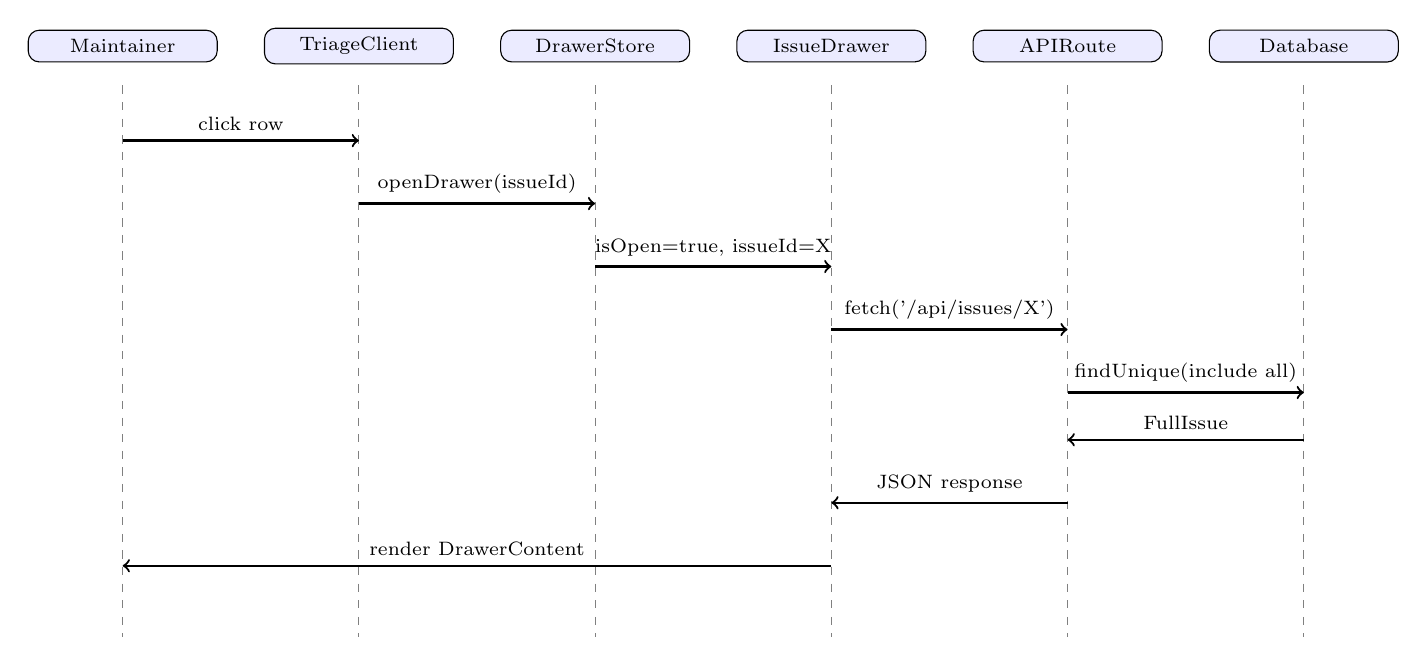
\begin{tikzpicture}[font=\small]
  \foreach \x/\name in {0/Maintainer,3/TriageClient,6/DrawerStore,9/IssueDrawer,12/APIRoute,15/Database}{
    \node[draw,fill=blue!8,rounded corners,minimum width=2.4cm,align=center,font=\scriptsize] at (\x,0) {\name};
    \draw[dashed,gray] (\x,-0.5) -- (\x,-7.5);
  }
  \draw[->,thick] (0,-1.2)  -- (3,-1.2)  node[midway,above,font=\scriptsize]{click row};
  \draw[->,thick] (3,-2.0)  -- (6,-2.0)  node[midway,above,font=\scriptsize]{openDrawer(issueId)};
  \draw[->,thick] (6,-2.8)  -- (9,-2.8)  node[midway,above,font=\scriptsize]{isOpen=true, issueId=X};
  \draw[->,thick] (9,-3.6)  -- (12,-3.6) node[midway,above,font=\scriptsize]{fetch('/api/issues/X')};
  \draw[->,thick] (12,-4.4) -- (15,-4.4) node[midway,above,font=\scriptsize]{findUnique(include all)};
  \draw[<-,thick] (12,-5.0) -- (15,-5.0) node[midway,above,font=\scriptsize]{FullIssue};
  \draw[<-,thick] (9,-5.8)  -- (12,-5.8) node[midway,above,font=\scriptsize]{JSON response};
  \draw[->,thick] (9,-6.6)  -- (0,-6.6)  node[midway,above,font=\scriptsize]{render DrawerContent};
\end{tikzpicture}
\caption{Sequence Diagram: Open Issue Drawer (D-SQ-03)}
\label{fig:sd-drawer}
\end{figure}

\subsubsection{SD-04: Bulk Spam}

\begin{figure}[H]
\centering
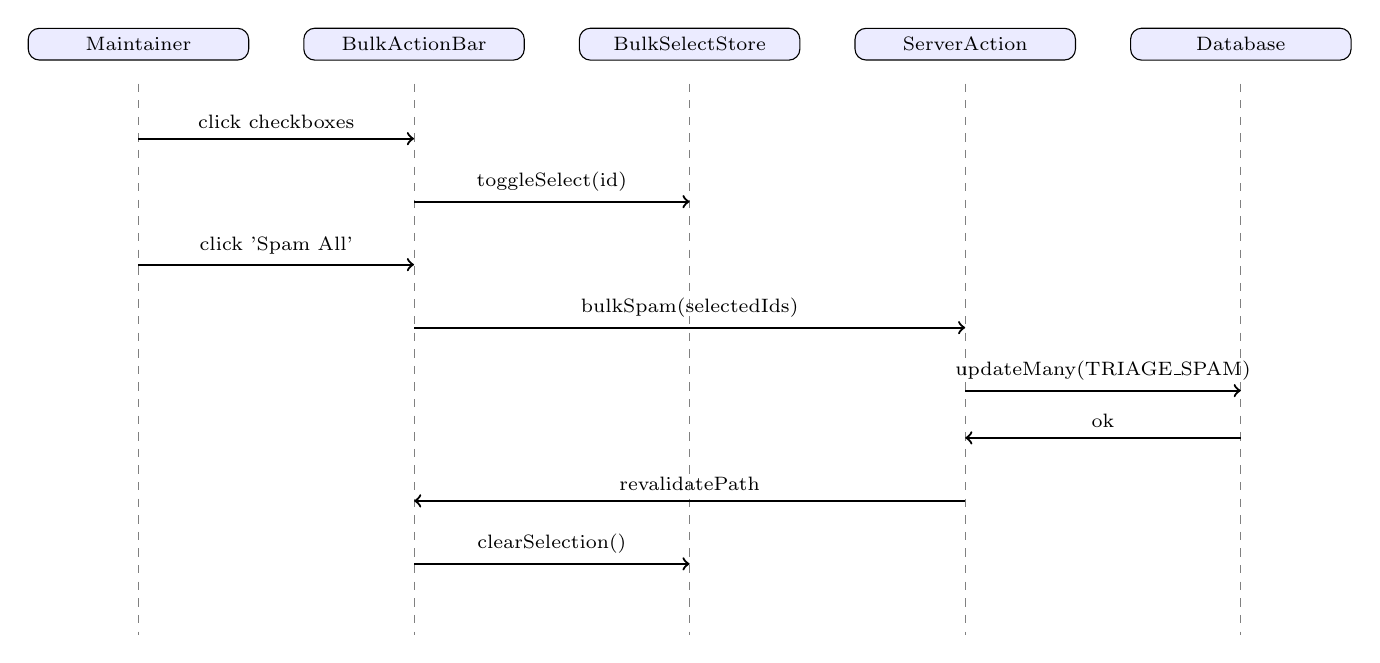
\begin{tikzpicture}[font=\small]
  \foreach \x/\name in {0/Maintainer,3.5/BulkActionBar,7/BulkSelectStore,10.5/ServerAction,14/Database}{
    \node[draw,fill=blue!8,rounded corners,minimum width=2.8cm,align=center,font=\scriptsize] at (\x,0) {\name};
    \draw[dashed,gray] (\x,-0.5) -- (\x,-7.5);
  }
  \draw[->,thick] (0,-1.2)    -- (3.5,-1.2)  node[midway,above,font=\scriptsize]{click checkboxes};
  \draw[->,thick] (3.5,-2.0)  -- (7,-2.0)    node[midway,above,font=\scriptsize]{toggleSelect(id)};
  \draw[->,thick] (0,-2.8)    -- (3.5,-2.8)  node[midway,above,font=\scriptsize]{click 'Spam All'};
  \draw[->,thick] (3.5,-3.6)  -- (10.5,-3.6) node[midway,above,font=\scriptsize]{bulkSpam(selectedIds)};
  \draw[->,thick] (10.5,-4.4) -- (14,-4.4)   node[midway,above,font=\scriptsize]{updateMany(TRIAGE\_SPAM)};
  \draw[<-,thick] (10.5,-5.0) -- (14,-5.0)   node[midway,above,font=\scriptsize]{ok};
  \draw[->,thick] (10.5,-5.8) -- (3.5,-5.8)  node[midway,above,font=\scriptsize]{revalidatePath};
  \draw[->,thick] (3.5,-6.6)  -- (7,-6.6)    node[midway,above,font=\scriptsize]{clearSelection()};
\end{tikzpicture}
\caption{Sequence Diagram: Bulk Spam (D-SQ-04)}
\label{fig:sd-bulk}
\end{figure}
\section{Database Schema}

Figure~\ref{fig:erd} presents the complete Entity-Relationship Diagram for the
CMS PostgreSQL database managed by Prisma.

\begin{figure}[H]
\centering
\resizebox{\textwidth}{!}{%
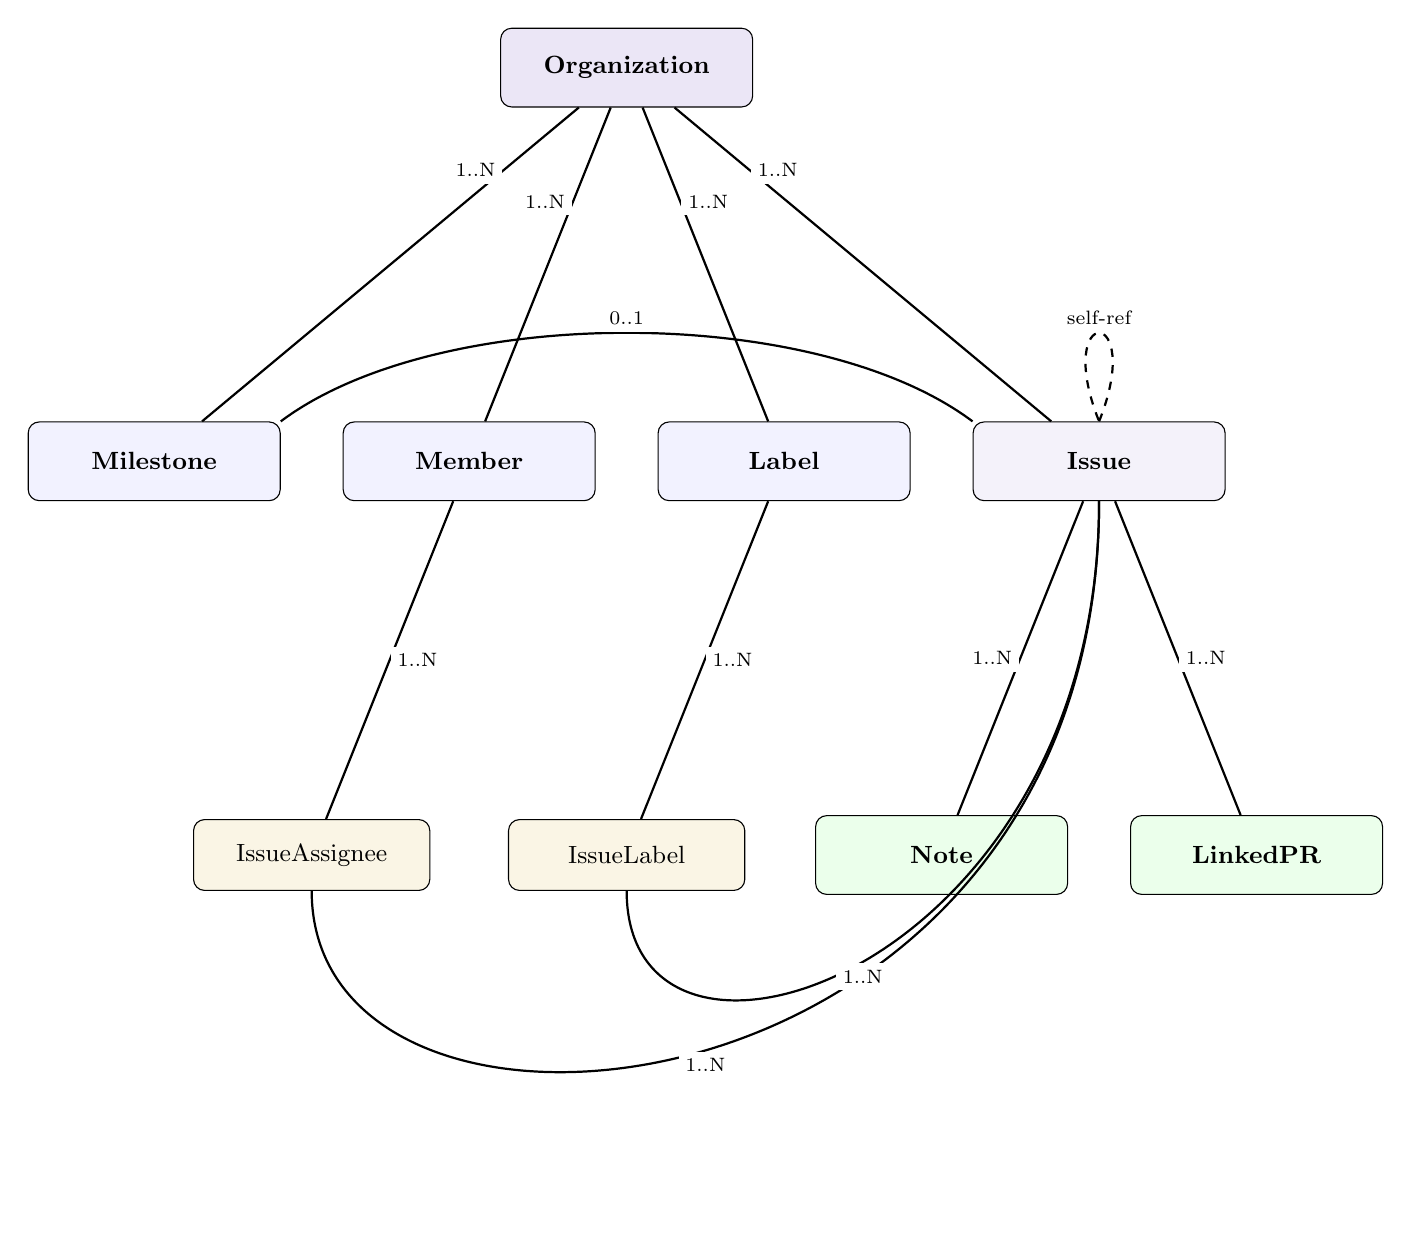
\begin{tikzpicture}[
  ent/.style={draw,fill=blue!5,rounded corners,minimum width=3.2cm,
              minimum height=1cm,align=center,font=\small\bfseries},
  jn/.style={draw,fill=warning!10,rounded corners,minimum width=3cm,
             minimum height=0.9cm,align=center,font=\small},
  arr/.style={-,thick},
  lbl/.style={font=\scriptsize,fill=white,inner sep=2.5pt}
]
%% ── Row 1: root ──────────────────────────────────────────────────────────────
\node[ent,fill=accent!15] (org) at (6, 0) {Organization};

%% ── Row 2: Org children ──────────────────────────────────────────────────────
%% Spread Member and Label close to their join tables (left side)
%% Keep Issue on the right with Note and LinkedPR below it
\node[ent]               (ms)  at (0, -5)  {Milestone};
\node[ent]               (mem) at (4, -5)  {Member};
\node[ent]               (lbl) at (8, -5)  {Label};
\node[ent,fill=accent!8] (iss) at (12,-5)  {Issue};

%% ── Row 3: leaf entities ─────────────────────────────────────────────────────
%% Join tables directly below their Org-side parent
\node[jn]               (ia)  at (2, -10) {IssueAssignee};
\node[jn]               (il)  at (6, -10) {IssueLabel};
%% Issue-owned directly below Issue
\node[ent,fill=green!8] (note)at (10,-10) {Note};
\node[ent,fill=green!8] (pr)  at (14,-10) {LinkedPR};

%% ── Org -> row-2 (labels near their own endpoints) ──────────────────────────
\draw[arr] (org) -- (ms)  node[lbl,pos=0.2,left]{1..N};
\draw[arr] (org) -- (mem) node[lbl,pos=0.3,left]{1..N};
\draw[arr] (org) -- (lbl) node[lbl,pos=0.3,right]{1..N};
\draw[arr] (org) -- (iss) node[lbl,pos=0.2,right]{1..N};

%% ── Milestone -> Issue (arc above row2, short hop between adjacent nodes) ───
\draw[arr] (ms.north east) .. controls +(2,1.5) and +(-2,1.5) .. (iss.north west)
  node[lbl,pos=0.5,above]{0..1};

%% ── Straight verticals: no crossing possible ─────────────────────────────────
\draw[arr] (mem) -- (ia)   node[lbl,midway,right]{1..N};
\draw[arr] (lbl) -- (il)   node[lbl,midway,right]{1..N};
\draw[arr] (iss) -- (note) node[lbl,midway,left]{1..N};
\draw[arr] (iss) -- (pr)   node[lbl,midway,right]{1..N};

%% ── Issue -> join tables: U-bends sweep BELOW row 3 (zero crossings) ─────────
\draw[arr] (iss.south) .. controls +(0,-8) and +(0,-4) .. (ia.south)
  node[lbl,pos=0.5,below]{1..N};
\draw[arr] (iss.south) .. controls +(0,-6) and +(0,-3) .. (il.south)
  node[lbl,pos=0.5,below]{1..N};

%% ── Self-ref: compact loop above Issue ───────────────────────────────────────
\draw[arr,dashed] (iss.north) .. controls +(0.6,1.5) and +(-0.6,1.5) ..
  (iss.north) node[lbl,pos=0.5,above]{self-ref};
\end{tikzpicture}%
}%% end resizebox
\caption{Entity-Relationship Diagram (D-DB-01)}
\label{fig:erd}
\end{figure}

\subsection{Enum Definitions}

\begin{longtable}{>{\bfseries}p{3cm} p{10cm}}
\toprule
Enum & Values \\
\midrule
\endhead
IssueSource & \texttt{DISCORD} | \texttt{GITHUB} \\
IssueStatus & \texttt{TRIAGE\_PENDING} | \texttt{TRIAGE\_SPAM} |
  \texttt{TRIAGE\_PROMOTED} | \texttt{BACKLOG} | \texttt{TODO} |
  \texttt{IN\_PROGRESS} | \texttt{IN\_REVIEW} | \texttt{DONE} |
  \texttt{CLOSED} \\
Priority & \texttt{NONE} | \texttt{LOW} | \texttt{MEDIUM} |
  \texttt{HIGH} | \texttt{CRITICAL} \\
\bottomrule
\end{longtable}

\subsection{Prisma Schema (Excerpt)}

\begin{lstlisting}[language=,caption={Core Issue model from schema.prisma}]
model Issue {
  id          String      @id @default(cuid())
  number      Int
  title       String
  body        String      @db.Text
  source      IssueSource
  status      IssueStatus @default(TRIAGE_PENDING)
  priority    Priority    @default(NONE)
  orgId       String
  org         Organization    @relation(...)

  // Discord metadata
  discordThreadId   String?
  discordAuthorName String?
  discordReplies    Json?

  // GitHub (post-promotion)
  githubIssueNumber Int?
  githubIssueUrl    String?
  linkedPRs         LinkedPR[]

  // AI deduplication
  similarityScore Float?
  duplicateOfId   String?
  duplicateOf     Issue?  @relation("Duplicates", ...)
  duplicates      Issue[] @relation("Duplicates")

  notes      Note[]
  createdAt  DateTime @default(now())
  updatedAt  DateTime @updatedAt
  lastActivityAt DateTime @default(now())

  @@unique([orgId, number])
}
\end{lstlisting}

\subsection{Issue Status Lifecycle}

\begin{figure}[H]
\centering
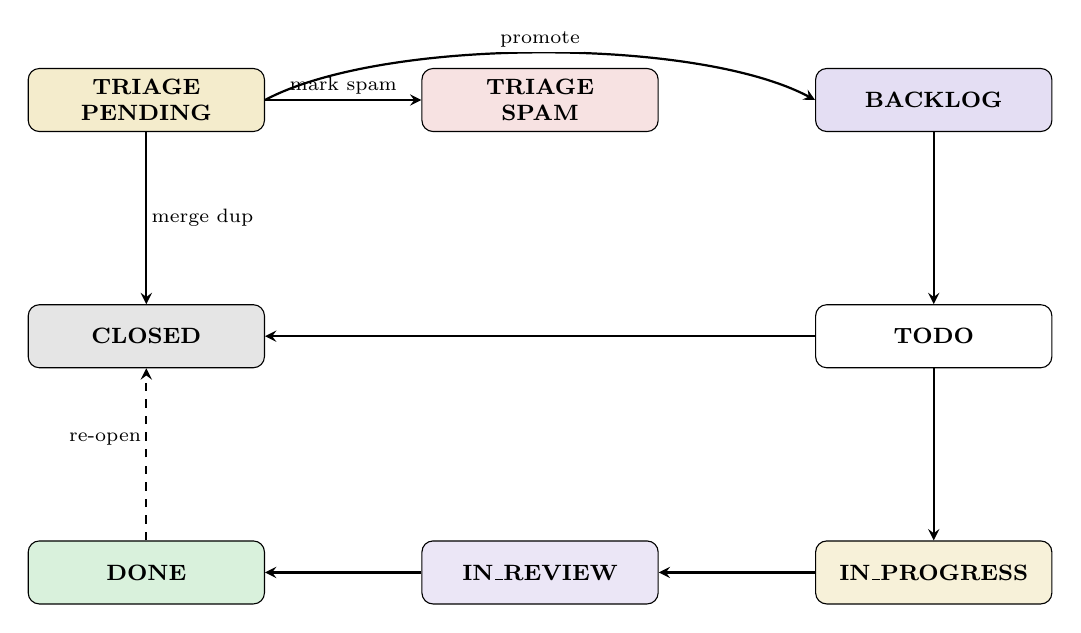
\begin{tikzpicture}[
  state/.style={draw,rounded corners,minimum width=3cm,minimum height=0.8cm,
                align=center,font=\footnotesize\bfseries},
  arr/.style={->,>=stealth,thick},
  lbl/.style={font=\scriptsize,fill=white,inner sep=1.5pt}
]
% Column 1 (x=0): PENDING -> DONE
% Column 2 (x=5): SPAM, BACKLOG
% Column 3 (x=10): TODO, IN_PROGRESS, IN_REVIEW
% Vertical rows: 0, -2.5, -5, -7.5
\node[state,fill=warning!20] (tp) at (0, 0)    {TRIAGE\\PENDING};
\node[state,fill=danger!15]  (ts) at (5, 0)    {TRIAGE\\SPAM};
\node[state,fill=accent!20]  (bl) at (10, 0)   {BACKLOG};
\node[state,fill=gray!20]    (cl) at (0,-3)    {CLOSED};
\node[state]                 (td) at (10,-3)   {TODO};
\node[state,fill=success!20] (dn) at (0,-6)    {DONE};
\node[state,fill=accent!15]  (ir) at (5,-6)    {IN\_REVIEW};
\node[state,fill=warning!15] (ip) at (10,-6)   {IN\_PROGRESS};

% Triage flow
\draw[arr] (tp) -- (ts)  node[lbl,midway,above]{mark spam};
\draw[arr] (tp.east) .. controls +(1.5,0.8) and +(-1.5,0.8) .. (bl.west)
  node[lbl,midway,above]{promote};
% Active board flow (right column, down)
\draw[arr] (bl) -- (td);
\draw[arr] (td) -- (ip);
\draw[arr] (ip) -- (ir);
\draw[arr] (ir) -- (dn);
% CLOSED transitions
\draw[arr] (tp) -- (cl)  node[lbl,midway,right]{merge dup};
\draw[arr] (td.west) -- (cl.east);
% Re-open (dashed, from DONE back up to BACKLOG via arc)
\draw[arr,dashed] (dn.north) .. controls +(0,1.5) and +(0,-1) .. (cl.south)
  node[lbl,pos=0.5,left]{re-open};
\end{tikzpicture}
\caption{Issue Status State Machine}
\label{fig:state-machine}
\end{figure}

\section{Security Design}

\subsection{Authentication and Authorization Mechanisms}

The current MVP employs a \textbf{mock session} strategy suitable for a local /
private-network deployment.  The \texttt{lib/mockSession.ts} module returns a
hardcoded maintainer identity.  In the planned production phase the following
mechanisms will be integrated:

\begin{enumerate}
  \item \textbf{NextAuth.js} with GitHub OAuth provider --- maintainers log in
    with their GitHub account.
  \item \textbf{Organisation Membership Verification} --- after OAuth, the
    system checks that the authenticated user is a member of the configured
    GitHub organisation via the GitHub API before granting dashboard access.
  \item \textbf{Role-Based Access} --- the \texttt{Member.role} field
    (currently always \texttt{"maintainer"}) will gate actions:
    \begin{itemize}
      \item \textbf{Viewer} --- read-only triage and board access.
      \item \textbf{Maintainer} --- promote, spam, label, assign.
      \item \textbf{Admin} --- settings, label creation, member management.
    \end{itemize}
  \item \textbf{Public Mirror} --- the read-only public interface requires no
    authentication; it queries a dedicated read replica with no write
    permissions.
\end{enumerate}

\subsection{Security Protocols}

\begin{longtable}{>{\bfseries}p{2.8cm} p{10cm}}
\toprule
Control (ID) & Description \\
\midrule
\endhead
D-SEC-01 & \textbf{Server-Only Secrets} --- \texttt{GITHUB\_TOKEN} and
  \texttt{DISCORD\_BOT\_TOKEN} are read exclusively inside Server Actions and
  API Route handlers.  They are never imported by client components.  Next.js
  statically analyses imports and will throw a build error if a server-only
  module is imported in a client component. \\
D-SEC-02 & \textbf{Server Actions as Secure Endpoints} --- All mutation
  operations (promote, spam, create, move) are implemented as \texttt{"use server"} functions.  The runtime enforces that these are called only from trusted
  server contexts. \\
D-SEC-03 & \textbf{Input Validation} --- The \texttt{validateTitleWordLimit()}
  function enforces a 200-word cap on all titles before any database write. \\
D-SEC-04 & \textbf{SQL Injection Prevention} --- All queries pass through
  Prisma's parameterised query builder.  No raw SQL is used in application code. \\
D-SEC-05 & \textbf{HTTPS/TLS} --- All external API calls (GitHub, Discord) use
  \texttt{https://} endpoints.  Production deployment must terminate TLS at the
  reverse proxy or CDN layer. \\
D-SEC-06 & \textbf{Cascade Delete Protection} --- Foreign-key cascade rules in
  the Prisma schema ensure that deleting an \texttt{Issue} automatically
  removes its \texttt{Note}, \texttt{IssueAssignee}, \texttt{IssueLabel}, and
  \texttt{LinkedPR} records, preventing orphan data accumulation. \\
D-SEC-07 & \textbf{No PII in URLs} --- The Issue Drawer fetches issue detail
  via \texttt{/api/issues/\{id\}} where \texttt{id} is an opaque CUID, not a
  user handle or email address. \\
D-SEC-08 & \textbf{Content Security} --- Discord \texttt{discordReplies} JSON
  is stored verbatim and rendered as plain text (\texttt{whitespace-pre-wrap}),
  not as \texttt{dangerouslySetInnerHTML}, preventing XSS injection from
  untrusted Discord content. \\
D-SEC-09 & \textbf{Grace-Degrade on Missing Credentials} --- Both
  \texttt{isGitHubIntegrationEnabled()} and \texttt{isDiscordBotEnabled()}
  check for the presence of env vars before attempting external API calls,
  preventing unhandled exceptions when credentials are absent. \\
\bottomrule
\end{longtable}
%% ============================================================
%%  5.0  TRACEABILITY
%% ============================================================
\chapter{Traceability}

\section{Requirement-to-Design Mapping}

The table below maps each functional requirement (FR), non-functional
requirement (NFR), and use case (UC) to the design artefacts that realise it.

\begin{longtable}{>{\bfseries}p{2.2cm} p{4.5cm} p{3.5cm} p{3.5cm}}
\toprule
Req./UC ID & Name & Design ID(s) & Design Artefact \\
\midrule
\endhead
UC-01 & Triage Discord Complaint & D-CL-01, D-CL-02, D-SQ-01 & Class Diagram, Sequence Diagram \\
UC-02 & Move Kanban Card & D-CL-02, D-SQ-02 & Class Diagram, Sequence Diagram \\
UC-03 & Bulk Spam Session & D-CL-02, D-SQ-04 & Class Diagram, Sequence Diagram \\
UC-04 & Create Internal Complaint & D-CL-01, D-CL-02 & Class Diagram \\
UC-05 & AI Duplicate Alert & D-CL-01, D-DB-01 & Class Diagram, ERD \\
FR-01 & List Discord Issues & D-CL-02 & Component Class Diagram \\
FR-02 & Filter Triage View & D-CL-02 & Component Class Diagram \\
FR-03 & Keyboard Navigation & D-CL-02 & Component Class Diagram \\
FR-04 & Promote Issue & D-CL-01, D-SQ-01 & Class Diagram, Sequence Diagram \\
FR-05 & Mark Spam & D-CL-01, D-SQ-04 & Class Diagram, Sequence Diagram \\
FR-06 & Mark Done & D-CL-01 & Class Diagram \\
FR-07 & Bulk Select & D-CL-02 & Component Class Diagram \\
FR-08 & Bulk Promote & D-CL-02, D-SQ-04 & Class Diagram, Sequence Diagram \\
FR-09 & Bulk Spam & D-CL-02, D-SQ-04 & Class Diagram, Sequence Diagram \\
FR-10 & Similarity Display & D-CL-01, D-DB-01 & Class Diagram, ERD \\
FR-11 & Display Board Columns & D-CL-02 & Component Class Diagram \\
FR-12 & Drag-and-Drop Cards & D-CL-02, D-SQ-02 & Class Diagram, Sequence Diagram \\
FR-13 & Card Metadata & D-CL-01, D-CL-02 & Class Diagram \\
FR-14 & Milestone Progress & D-CL-01, D-DB-01 & Class Diagram, ERD \\
FR-15 & Move Status Persist & D-CL-01, D-SQ-02 & Class Diagram, Sequence Diagram \\
FR-16 & Fetch Issue Detail & D-CL-02, D-SQ-03 & Class Diagram, Sequence Diagram \\
FR-17 & Discord Thread View & D-CL-01, D-CL-02 & Class Diagram \\
FR-18 & AI Similarity Block & D-CL-01, D-DB-01 & Class Diagram, ERD \\
FR-19 & Dual Chat Tabs & D-CL-02 & Component Class Diagram \\
FR-20 & Focus Mode & D-CL-02 & Component Class Diagram \\
FR-21 & Promote from Drawer & D-CL-02, D-SQ-01 & Class Diagram, Sequence Diagram \\
FR-22 & Copy Link & D-CL-02 & Component Class Diagram \\
FR-23 & Metadata Sidebar & D-CL-01, D-CL-02 & Class Diagram \\
FR-24 & Create GitHub Issue & D-CL-01, D-SQ-01 & Class Diagram, Sequence Diagram \\
FR-25 & Discord Notification & D-CL-01, D-SQ-01 & Class Diagram, Sequence Diagram \\
FR-26 & Label Retry & D-CL-01 & Class Diagram \\
FR-27 & Status Update & D-CL-01, D-DB-01 & Class Diagram, ERD \\
FR-28 & Open Create Modal & D-CL-02 & Component Class Diagram \\
FR-29 & Validate Title & D-CL-01 & Class Diagram \\
FR-30 & Persist Complaint & D-CL-01, D-DB-01 & Class Diagram, ERD \\
FR-31 & Post-Create Navigation & D-CL-02 & Component Class Diagram \\
FR-32 & Open Palette & D-CL-02 & Component Class Diagram \\
FR-33 & Navigate Commands & D-CL-02 & Component Class Diagram \\
FR-34 & Go-to Sequences & D-CL-02 & Component Class Diagram \\
NFR-01 & Performance & D-CL-02 & Component Class Diagram (RSC data fetch) \\
NFR-02 & Security (Server Actions) & D-SEC-02 & Security List \\
NFR-03 & Security (Secrets) & D-SEC-01 & Security List \\
NFR-04 & Reliability (Optimistic UI) & D-SQ-02 & Sequence Diagram \\
NFR-05 & Keyboard Usability & D-CL-02 & Component Class Diagram \\
NFR-06 & Scalability (N+1) & D-DB-01 & ERD / Prisma includes \\
NFR-07 & TypeScript Strict & D-CL-01, D-CL-02 & Class Diagrams \\
NFR-08 & Accessibility & D-CL-02 & Component Class Diagram \\
NFR-09 & Deployability & --- & Deployment Section \\
NFR-10 & Data Integrity (Cascade) & D-DB-01, D-SEC-06 & ERD, Security List \\
\bottomrule
\end{longtable}

%% ============================================================
%%  6.0  CODE
%% ============================================================
\chapter{Code}

\section{Repository}

The complete source code for the Complaint Management System is hosted on
GitHub.  The repository contains the full Next.js application, Prisma schema,
Docker scripts, and documentation.

\begin{tcolorbox}[colback=gray!6,colframe=accent!50,boxrule=0.6pt]
\textbf{Repository URL:}\\[0.5em]
\texttt{https://github.com/Unique-45/Complaint-Management-System}\\[1em]
\textbf{Default Branch:} \texttt{main}\quad\textbf{License:} MIT
\end{tcolorbox}

\section{Repository Structure}

\begin{lstlisting}[caption={Project directory tree (key files)}]
complaint-management-system/
|-- src/
|   |-- app/
|   |   |-- api/issues/[id]/route.ts    # REST endpoint for drawer
|   |   |-- dashboard/
|   |   |   |-- layout.tsx              # DashboardLayout RSC
|   |   |   |-- triage/page.tsx         # Triage Inbox page
|   |   |   |-- board/page.tsx          # Kanban Board page
|   |   |   `-- settings/page.tsx
|   |-- components/
|   |   |-- triage/TriageClient.tsx     # Triage table (client)
|   |   |-- board/KanbanBoard.tsx       # DnD Kanban (client)
|   |   |-- drawer/IssueDrawer.tsx      # Slide-over drawer (client)
|   |   |-- layout/                     # Sidebar, TopBar, KeyboardHandler
|   |   `-- issue/CreateIssueModal.tsx
|   |-- server/actions/issues.ts        # All server actions
|   |-- lib/
|   |   |-- prisma.ts                   # Prisma client singleton
|   |   |-- utils.ts                    # Shared helpers & metadata
|   |   `-- integrations/
|   |       |-- github.ts               # GitHub API client
|   |       `-- discord.ts              # Discord API client
|   `-- stores/                         # Zustand client stores
|       |-- drawerStore.ts
|       |-- bulkSelectStore.ts
|       `-- triageCursorStore.ts
|-- prisma/
|   |-- schema.prisma                   # Database schema
|   `-- seed.ts                         # Demo data seeder
|-- scripts/                            # db-up, db-reset, setup-local
|-- docker-compose.yml
|-- next.config.ts
`-- package.json
\end{lstlisting}

\section{GitHub Repository \& Commit History}

The project is hosted publicly at:
\begin{center}
  \texttt{\url{https://github.com/Unique-45/Complaint\_Management\_System}}
\end{center}

\subsection{Repository Overview}
\begin{figure}[H]
\centering
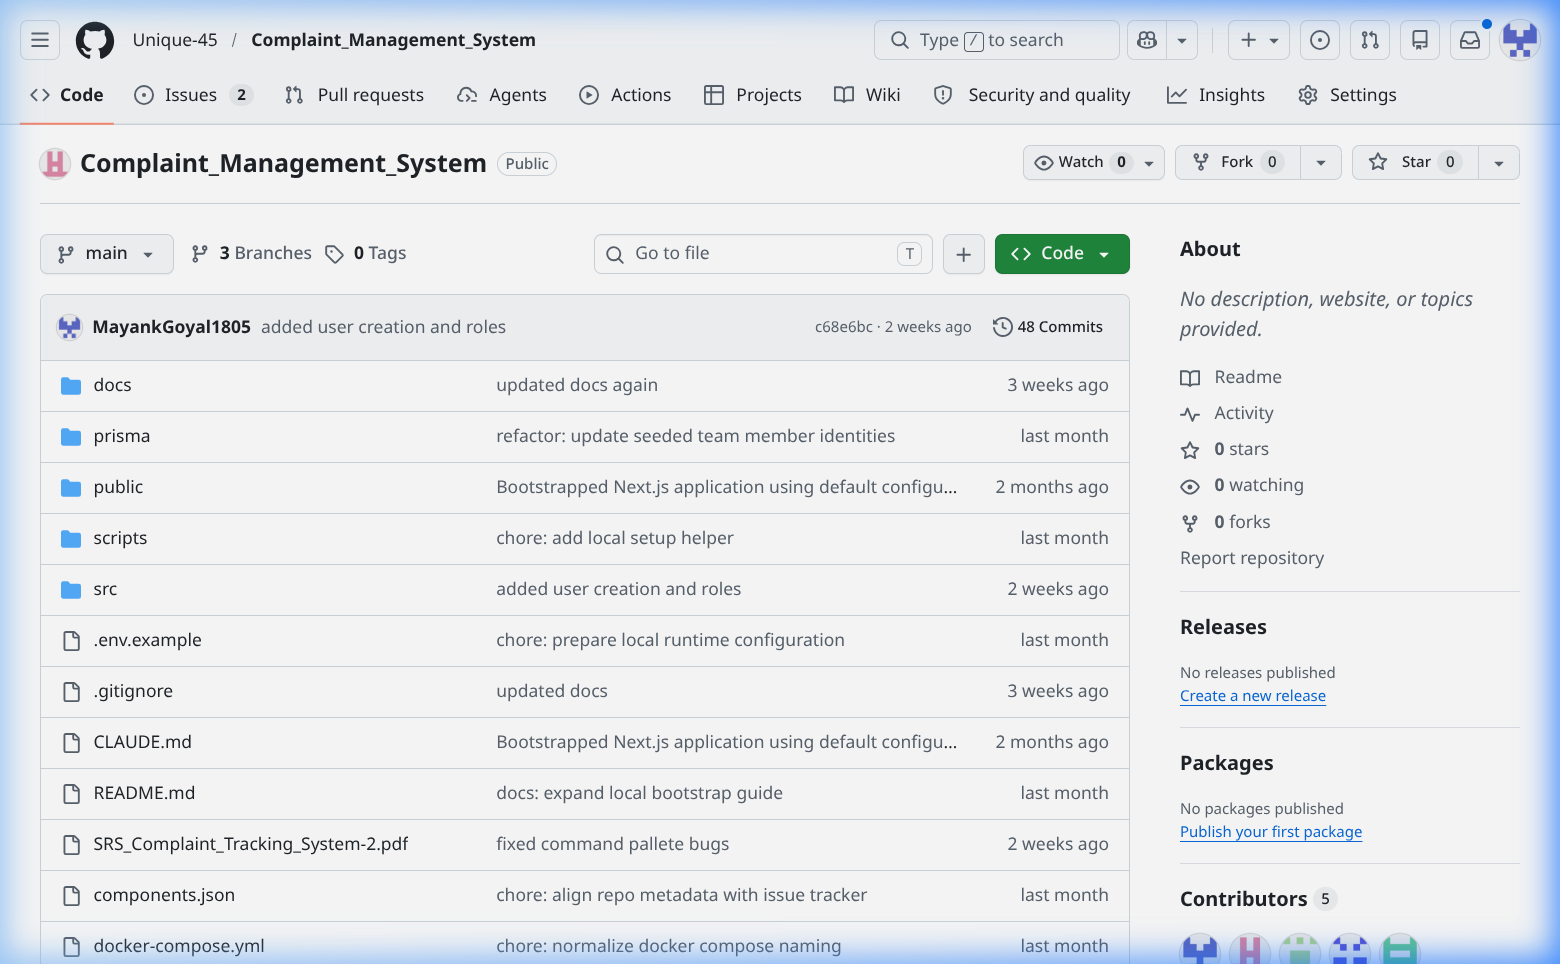
\includegraphics[width=\linewidth]{images/github_repo_main.png}
\caption{GitHub Repository --- project structure and README on the \texttt{main} branch}
\label{fig:gh-repo}
\end{figure}

\subsection{Contributor Activity Graph}
\begin{figure}[H]
\centering
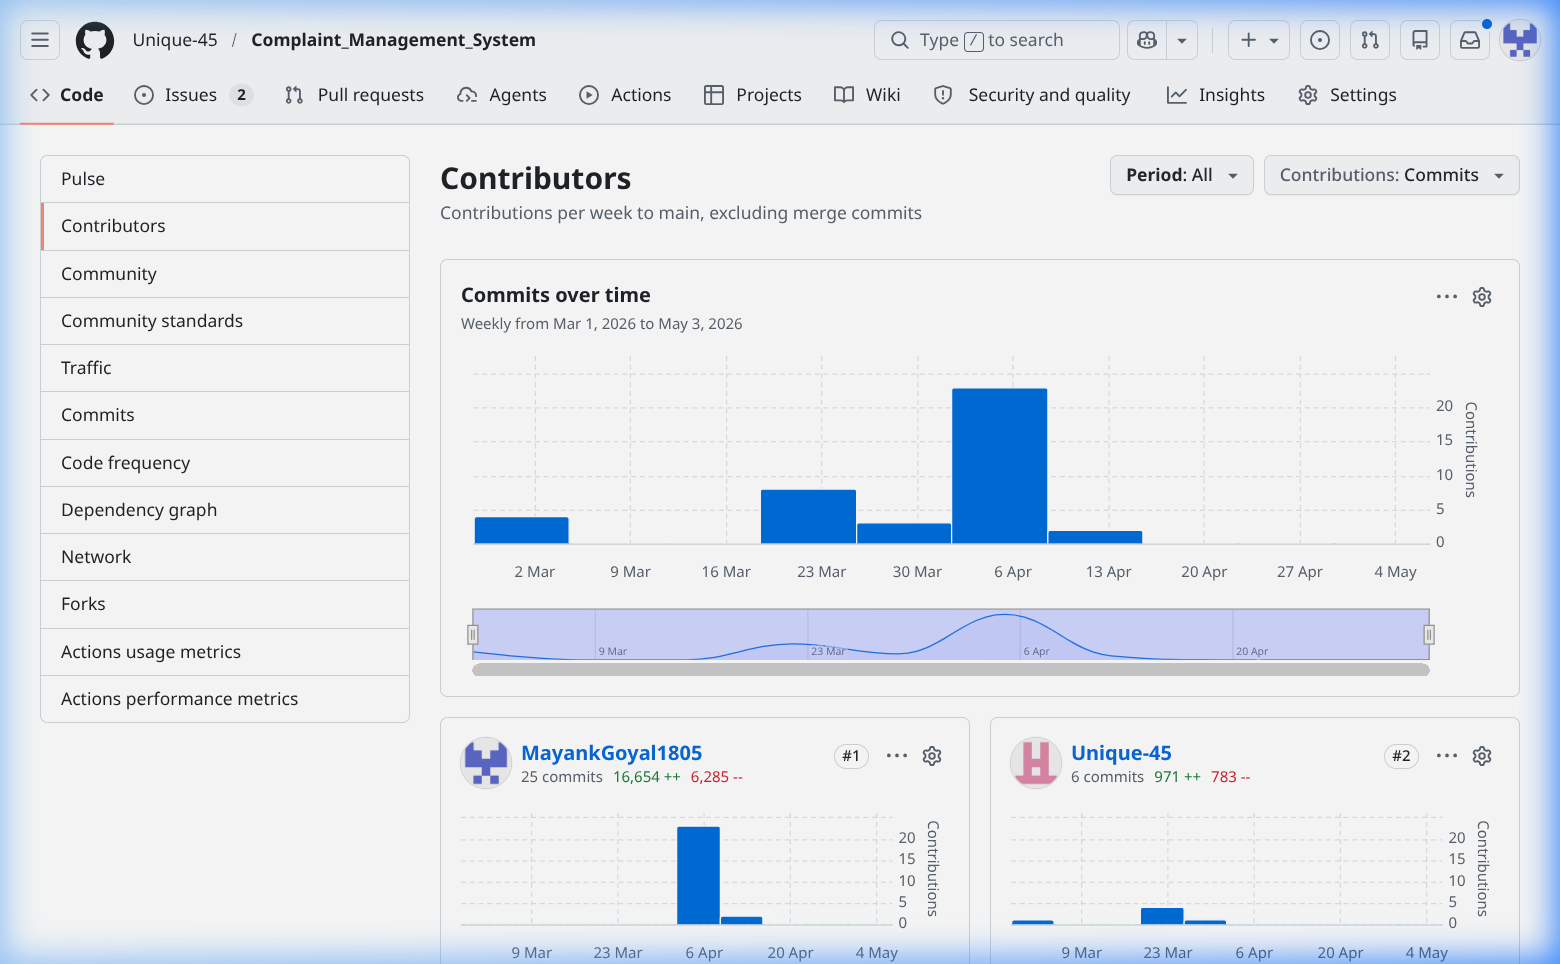
\includegraphics[width=\linewidth]{images/github_contributors.png}
\caption{GitHub Insights --- contributor activity across the full project timeline}
\label{fig:gh-contributors}
\end{figure}

%% ── Per-member commit histories ──────────────────────────────────────────────

\subsection{Individual Commit Histories}

\subsubsection*{Mayank Goyal \quad\normalfont\small(\texttt{mayankgoyal1805})}
\begin{figure}[H]
\centering
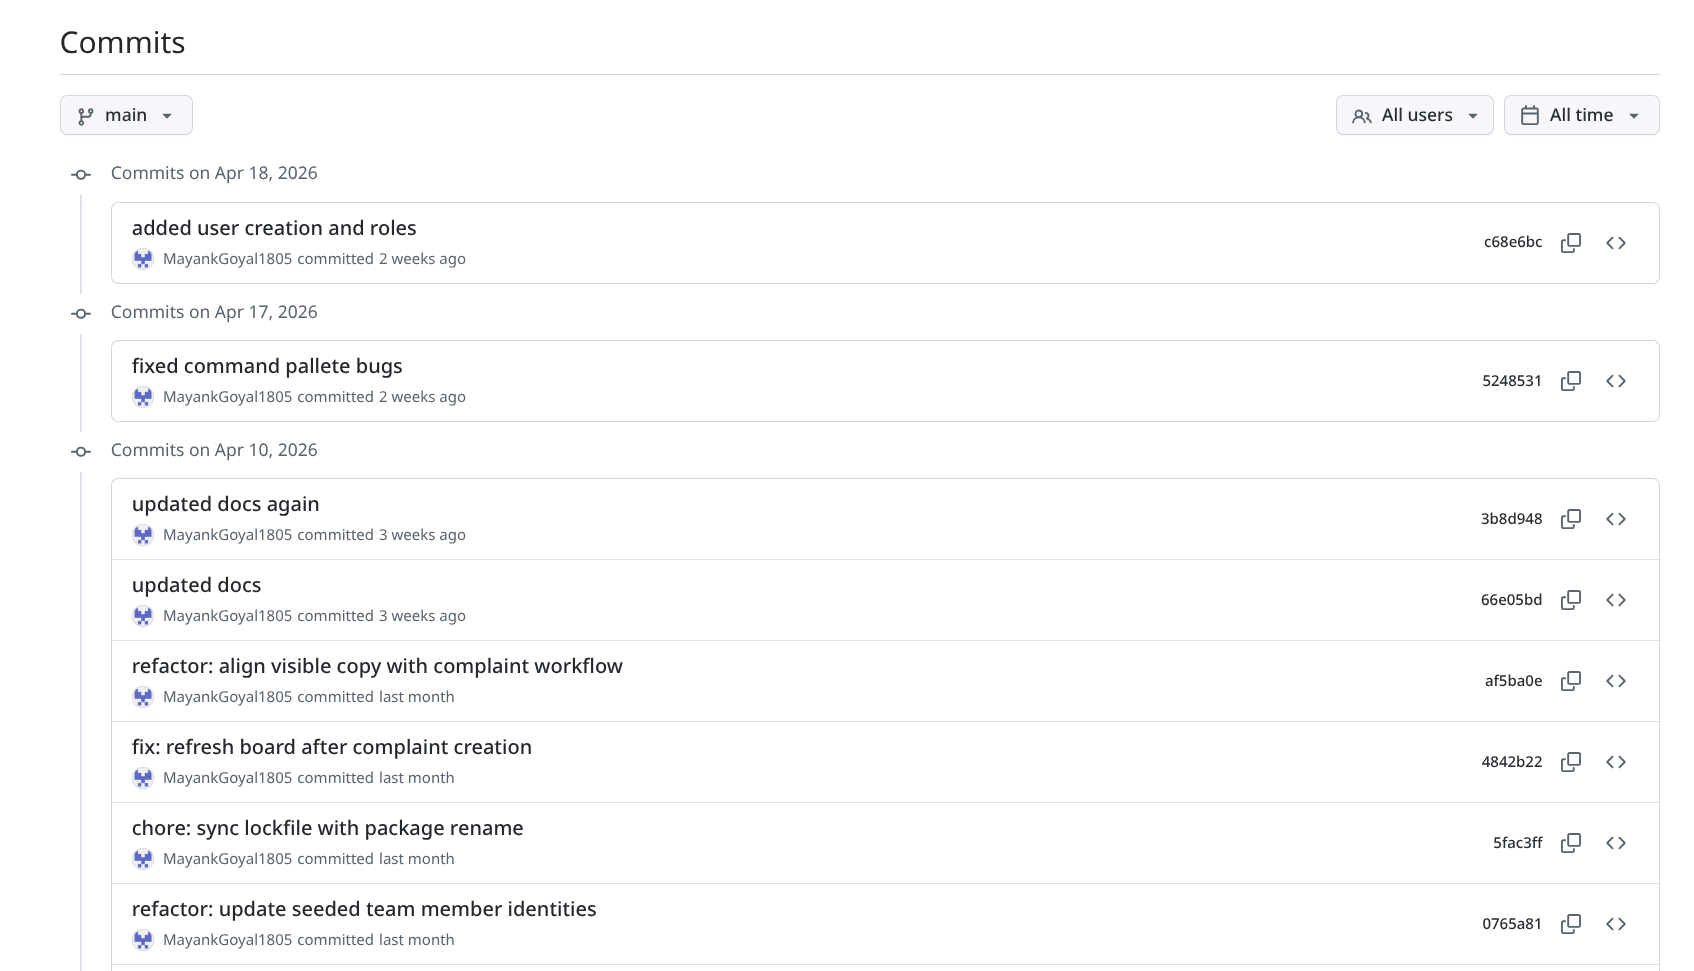
\includegraphics[width=\linewidth]{images/mayank1.png}
\caption{Mayank Goyal commits --- page 1}
\label{fig:c-mayank-1}
\end{figure}
\begin{figure}[H]
\centering
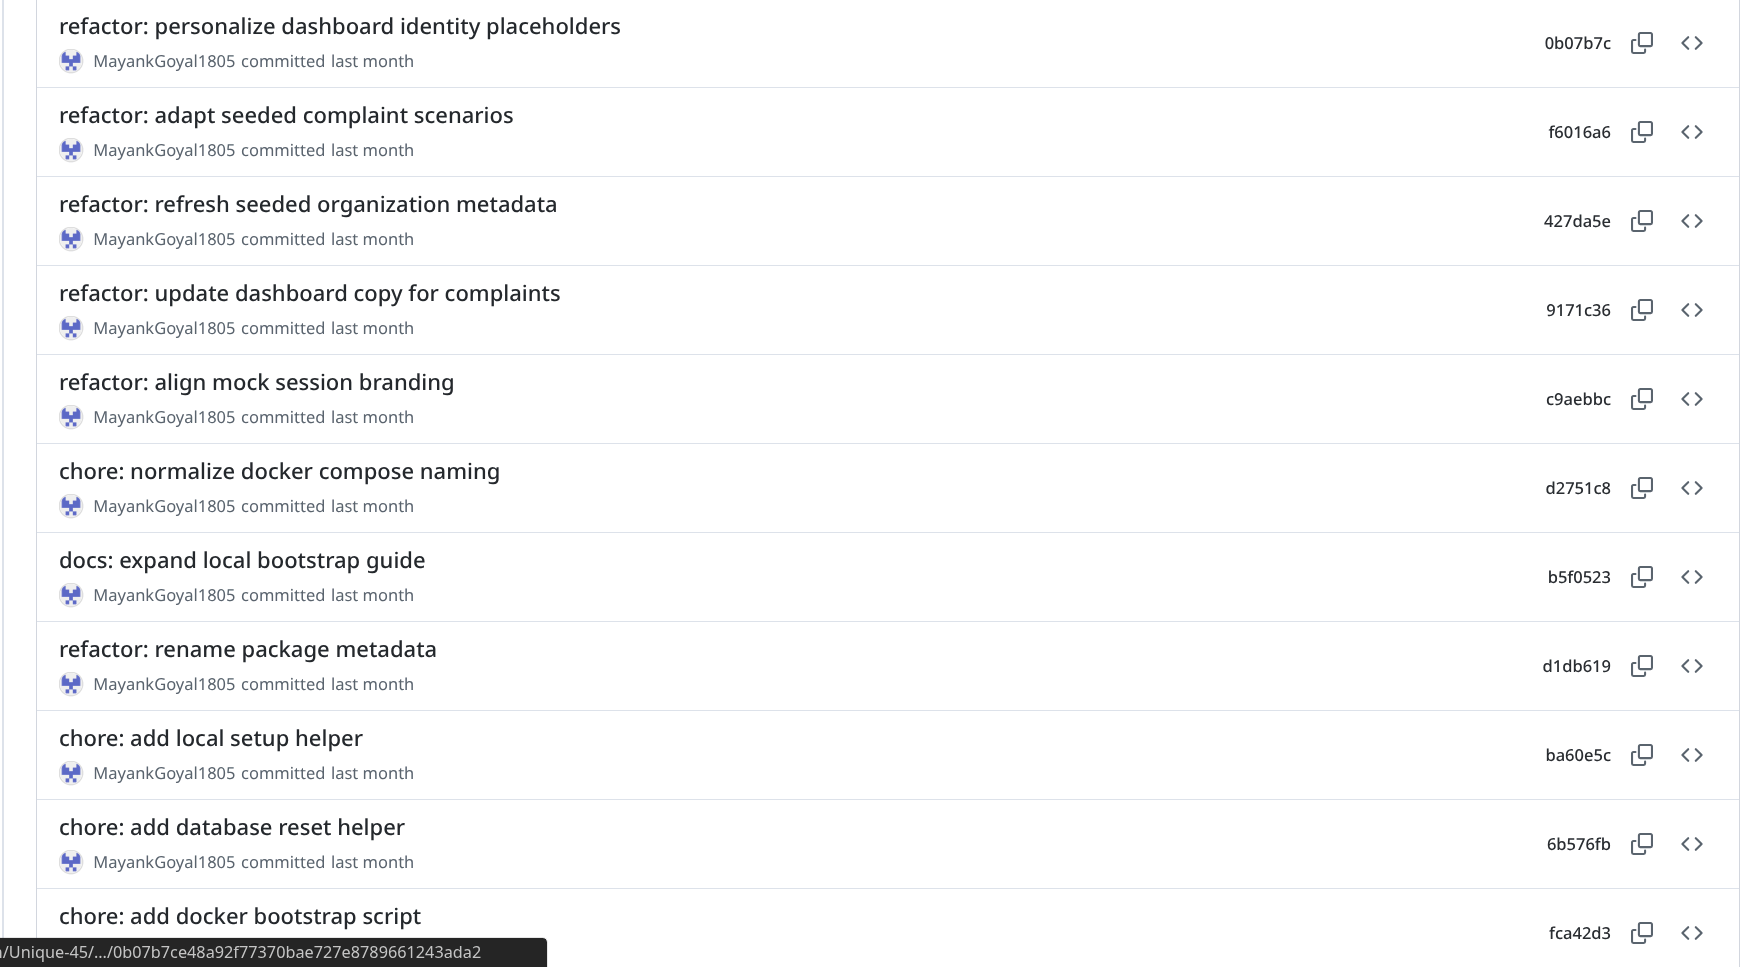
\includegraphics[width=\linewidth]{images/mayank2.png}
\caption{Mayank Goyal commits --- page 2}
\label{fig:c-mayank-2}
\end{figure}
\begin{figure}[H]
\centering
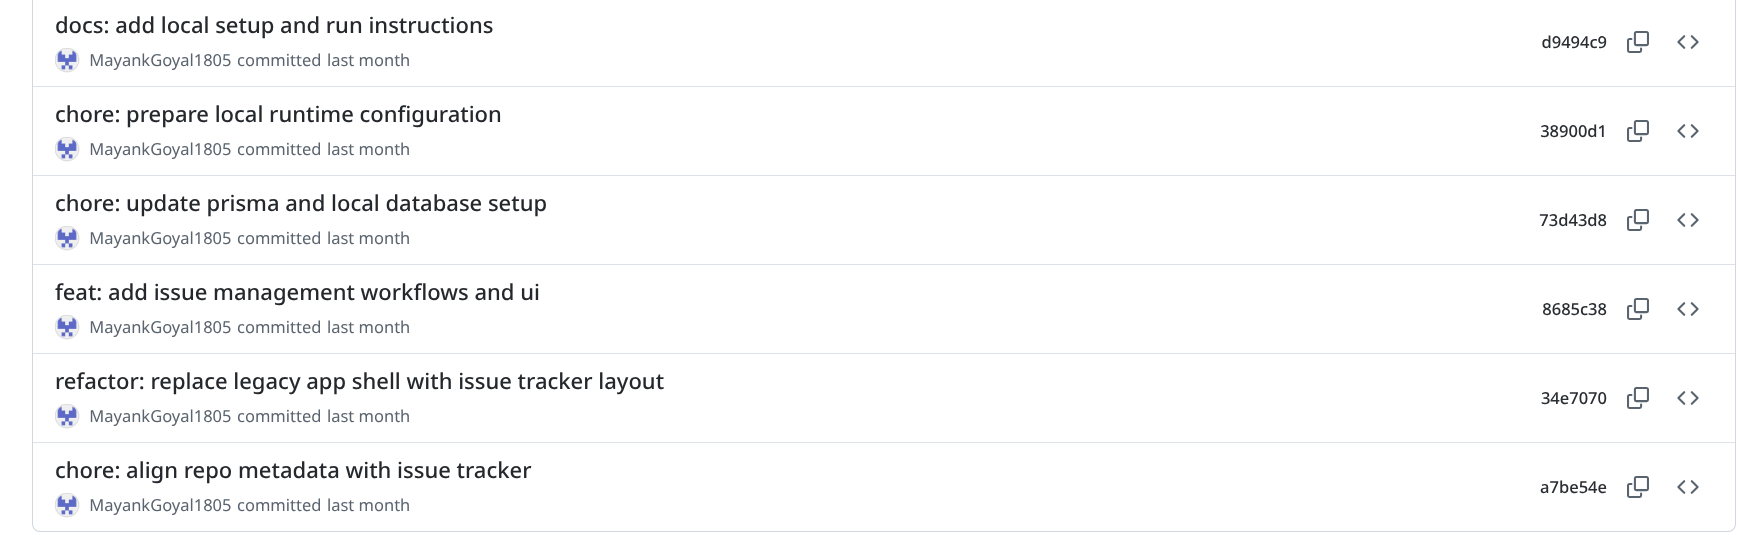
\includegraphics[width=\linewidth]{images/mayank3.png}
\caption{Mayank Goyal commits --- page 3}
\label{fig:c-mayank-3}
\end{figure}

\subsubsection*{Vansh Sahrawat \quad\normalfont\small(\texttt{Unique-45})}
\begin{figure}[H]
\centering
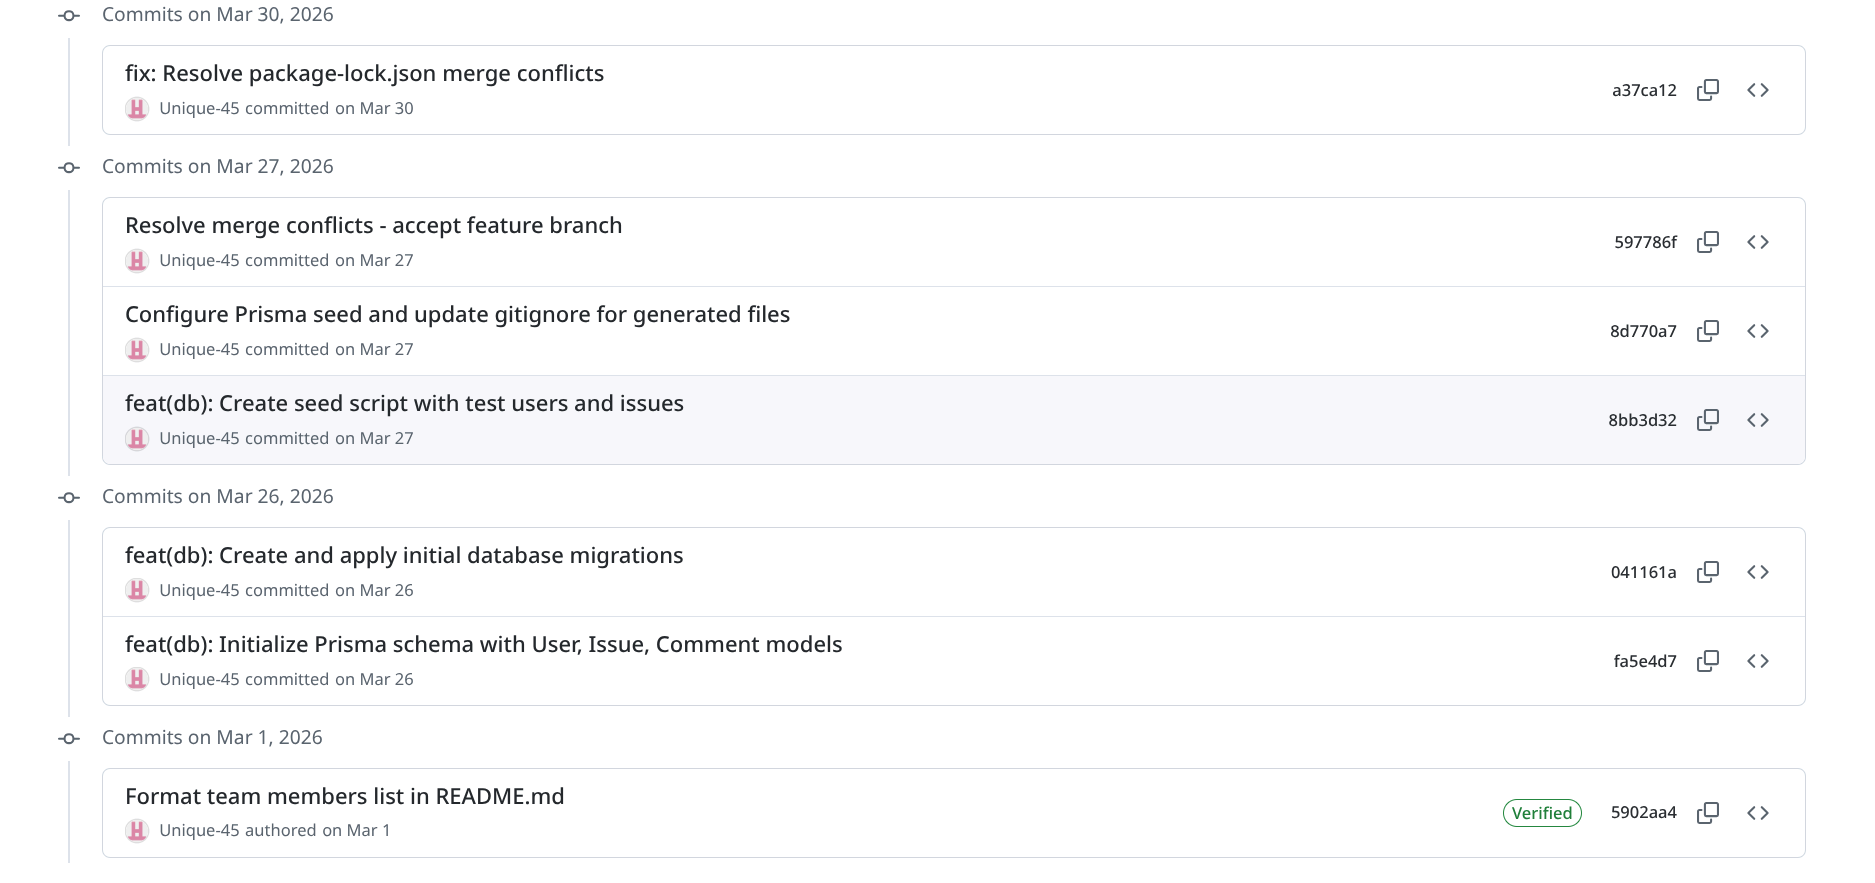
\includegraphics[width=\linewidth]{images/vansh1.png}
\caption{Vansh Sahrawat commits (Unique-45)}
\label{fig:c-vansh-1}
\end{figure}

\subsubsection*{Deepanshu Sharma \quad\normalfont\small(\texttt{deepanshu-shar})}
\begin{figure}[H]
\centering
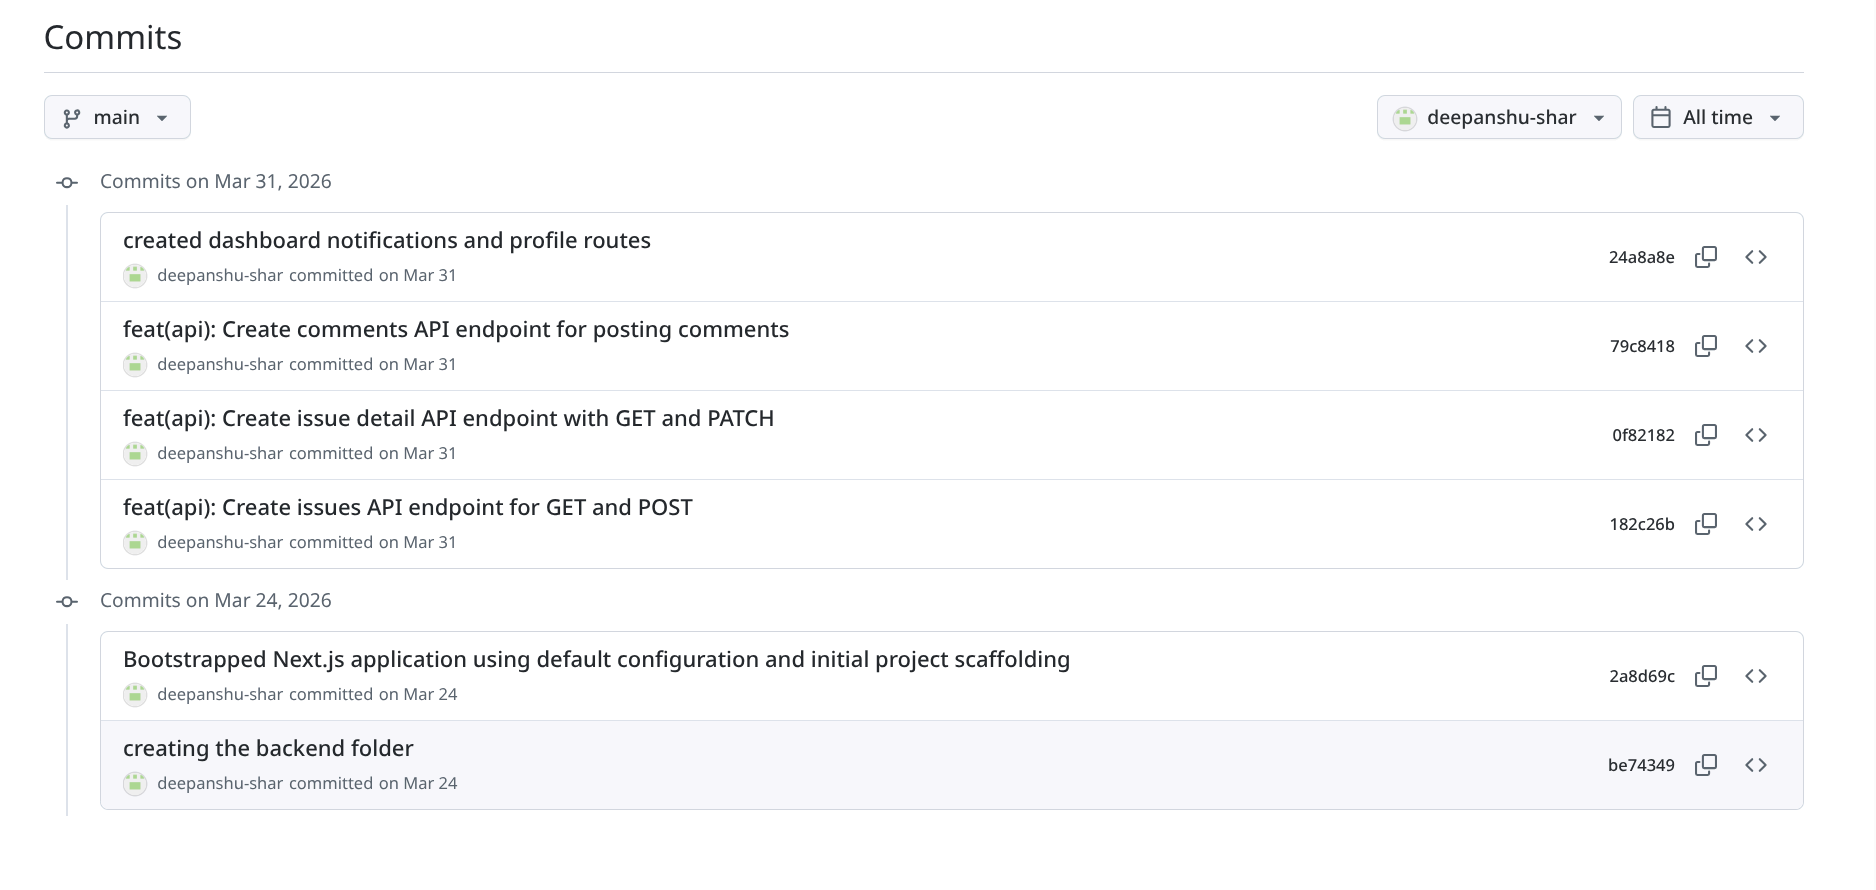
\includegraphics[width=\linewidth]{images/deepanshu1.png}
\caption{Deepanshu Sharma commits (deepanshu-shar)}
\label{fig:c-deepanshu-1}
\end{figure}

\subsubsection*{Krishan Kumar \quad\normalfont\small(\texttt{krishan1707})}
\begin{figure}[H]
\centering

\includegraphics[width=\linewidth]{images/krishan1.png}
\caption{Krishan Kumar commits (krishan1707)}
\label{fig:c-krishan-1}
\end{figure}

\subsubsection*{Prateek Binjola \quad\normalfont\small(\texttt{prateekbinjola})}
\begin{figure}[H]
\centering
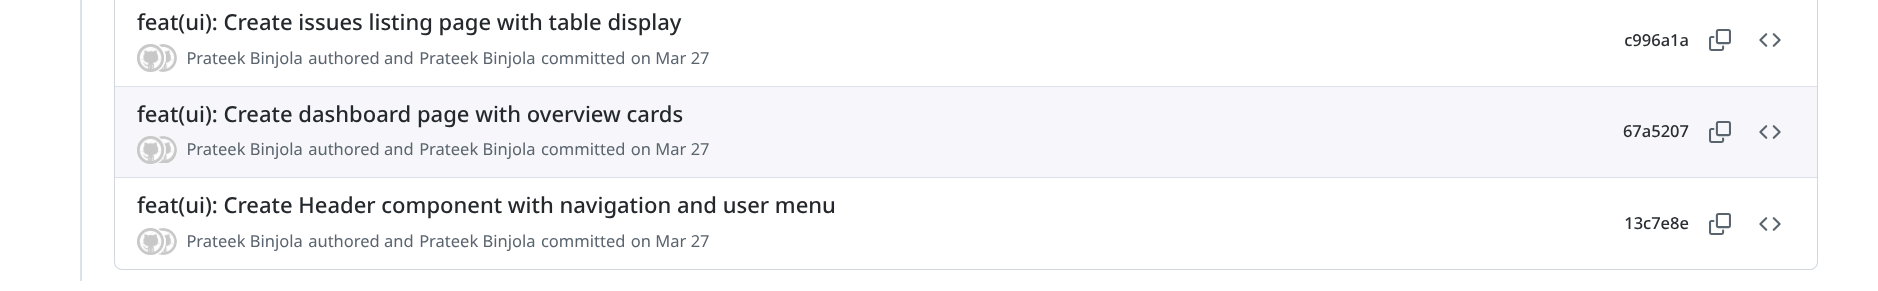
\includegraphics[width=\linewidth]{images/prateek1.png}
\caption{Prateek Binjola commits (prateekbinjola)}
\label{fig:c-prateek-1}
\end{figure}



%% ============================================================
%%  7.0  DEPLOYMENT
%% ============================================================
\chapter{Deployment}

\section{Deployment Architecture}

\begin{figure}[H]
\centering
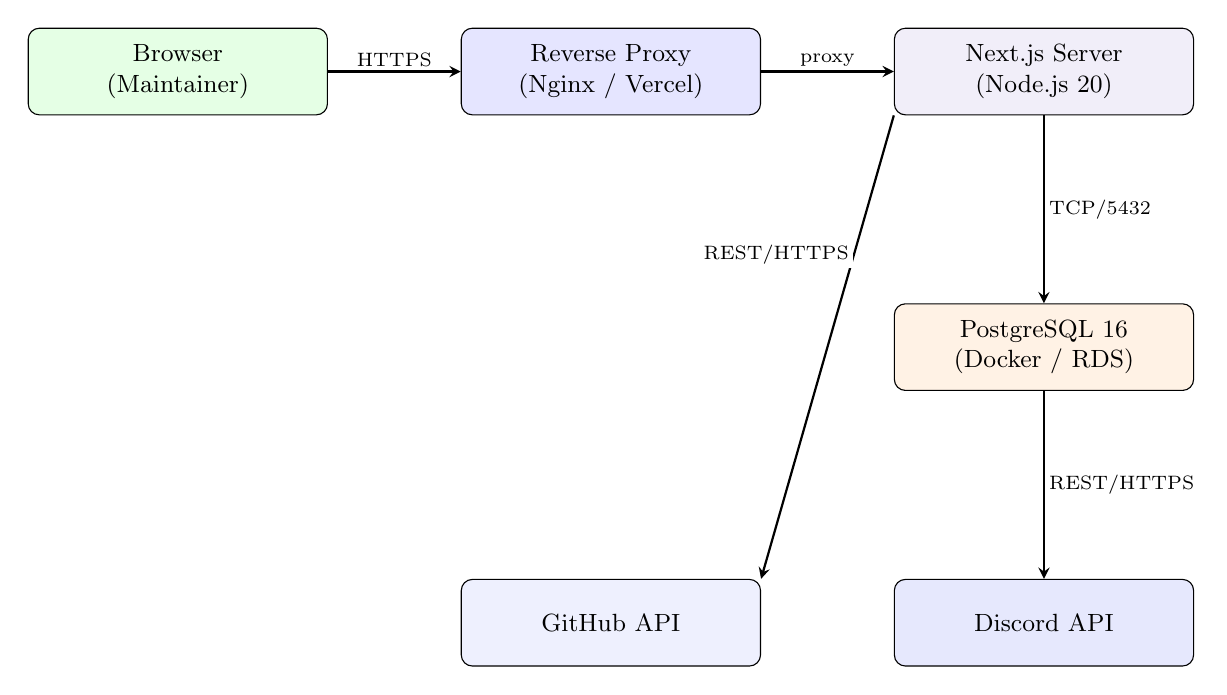
\begin{tikzpicture}[
  box/.style={draw,rounded corners,fill=blue!5,minimum width=3.8cm,
              minimum height=1.1cm,align=center,font=\small},
  arr/.style={->,>=stealth,thick},
  lbl/.style={font=\scriptsize,fill=white,inner sep=1.5pt}
]
% Row 1: Browser -> Proxy -> Next.js (spread wider)
\node[box,fill=green!10]  (user)  at (0,0)     {Browser\\(Maintainer)};
\node[box,fill=blue!10]   (nginx) at (5.5,0)   {Reverse Proxy\\(Nginx / Vercel)};
\node[box,fill=accent!10] (next)  at (11,0)    {Next.js Server\\(Node.js 20)};
% Row 2: DB under Next.js
\node[box,fill=orange!10] (pg)    at (11,-3.5) {PostgreSQL 16\\(Docker / RDS)};
% Row 3: External APIs
\node[box,fill=discord!10](gh)    at (5.5,-7)  {GitHub API};
\node[box,fill=discord!15](dc)    at (11,-7)   {Discord API};

% Horizontal flow (labels above, clear of nodes)
\draw[arr] (user)  -- (nginx) node[lbl,midway,above]{HTTPS};
\draw[arr] (nginx) -- (next)  node[lbl,midway,above]{proxy};
% Vertical: Next -> DB
\draw[arr] (next)  -- (pg)    node[lbl,midway,right]{TCP/5432};
% Next -> GitHub: diagonal, label placed off the line
\draw[arr] (next.south west) -- (gh.north east)
  node[lbl,pos=0.3,left]{REST/HTTPS};
% Next -> Discord: vertical
\draw[arr] (pg)    -- (dc)    node[lbl,midway,right]{REST/HTTPS};
\end{tikzpicture}
\caption{Production Deployment Architecture}
\label{fig:deployment}
\end{figure}

\section{Local Development Setup}

\begin{lstlisting}[language=bash,caption={Complete local bootstrap}]
# 1. Clone repository
git clone https://github.com/[org]/complaint-management-system
cd complaint-management-system

# 2. Install dependencies
npm install

# 3. Configure environment
cp .env.example .env
# Edit .env with your DATABASE_URL, GITHUB_TOKEN, DISCORD_BOT_TOKEN

# 4. One-command bootstrap (starts Docker, pushes schema, seeds data)
npm run setup

# 5. Start development server
npm run dev
# App available at http://localhost:3000
\end{lstlisting}

\section{Environment Variables}

\begin{longtable}{>{\ttfamily\bfseries}p{4.5cm} p{8cm}}
\toprule
Variable & Purpose \\
\midrule
\endhead
DATABASE\_URL & PostgreSQL connection string. \\
GITHUB\_TOKEN & GitHub Personal Access Token (repo scope). \\
GITHUB\_OWNER & GitHub organisation or user owning the target repo. \\
GITHUB\_REPO & Repository name to create issues in. \\
DISCORD\_BOT\_TOKEN & Discord Bot token for posting thread replies. \\
\bottomrule
\end{longtable}

\section{Screenshots of the Working Application}

\begin{tcolorbox}[colback=gray!5,colframe=gray!40,title=Instructions]
Run the application locally with \texttt{npm run dev} after seeding demo data
(\texttt{npm run db:seed}) and capture the following screenshots to insert
below.
\end{tcolorbox}

\vspace{1em}
\noindent\textbf{Screenshot 1 --- Triage Inbox}\\[0.5em]
\begin{figure}[H]
\centering
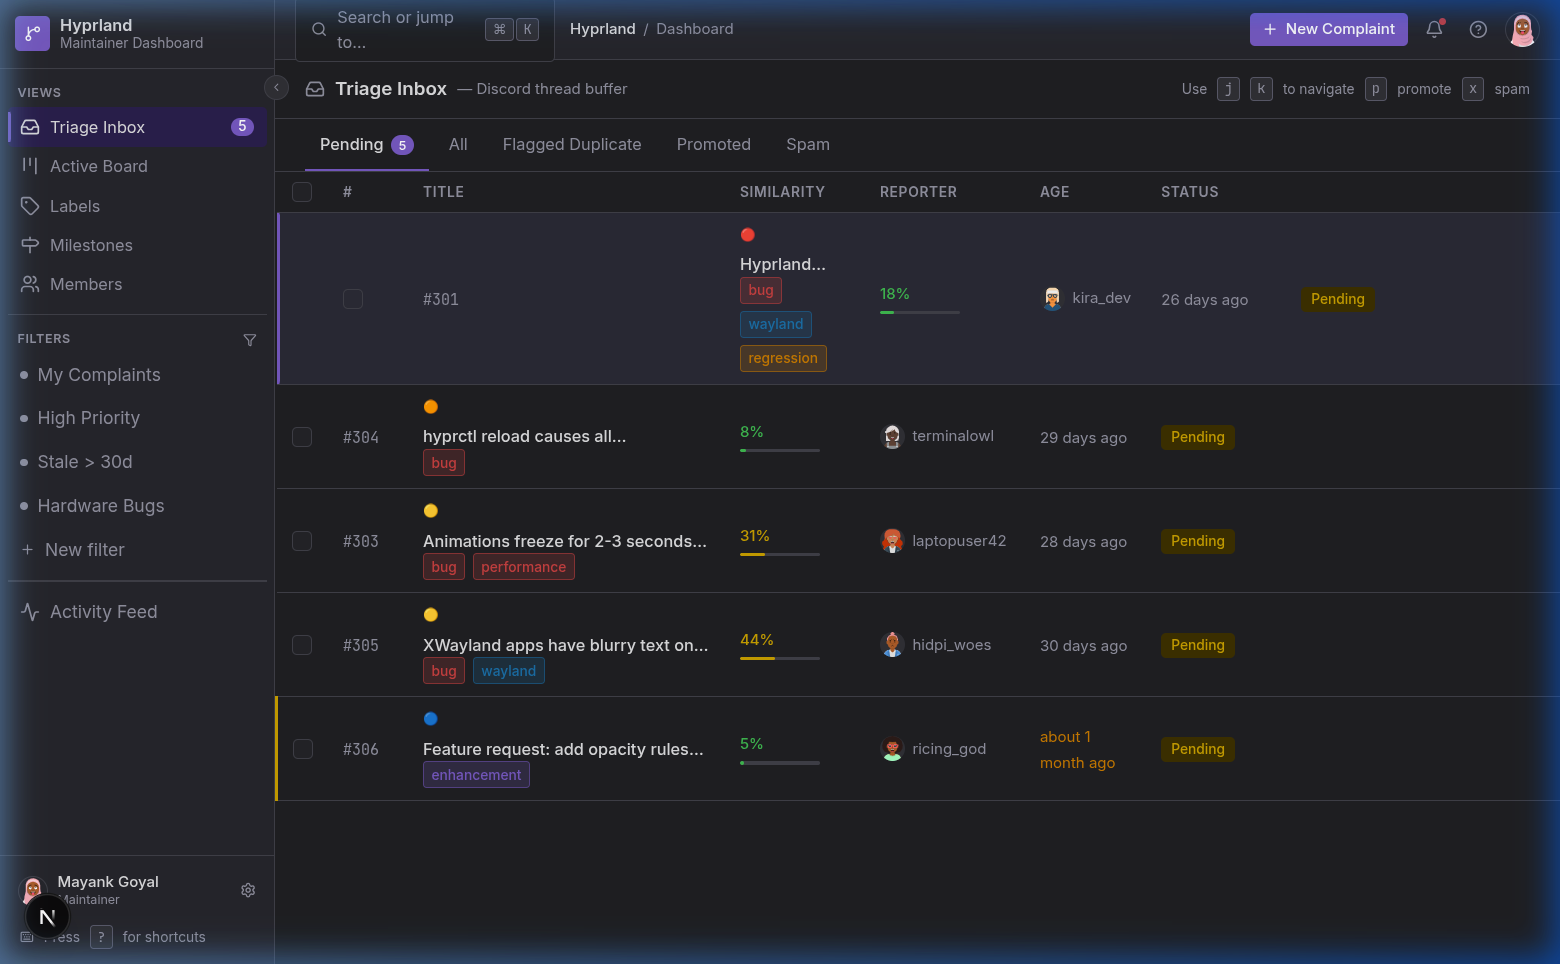
\includegraphics[width=\linewidth]{images/screenshot_triage.png}
\caption{Triage Inbox --- issue list with priority, source badges and action buttons}
\label{fig:ss-triage}
\end{figure}

\vspace{0.5em}
\noindent\textbf{Screenshot 2 --- Kanban Board}\\[0.5em]
\begin{figure}[H]
\centering
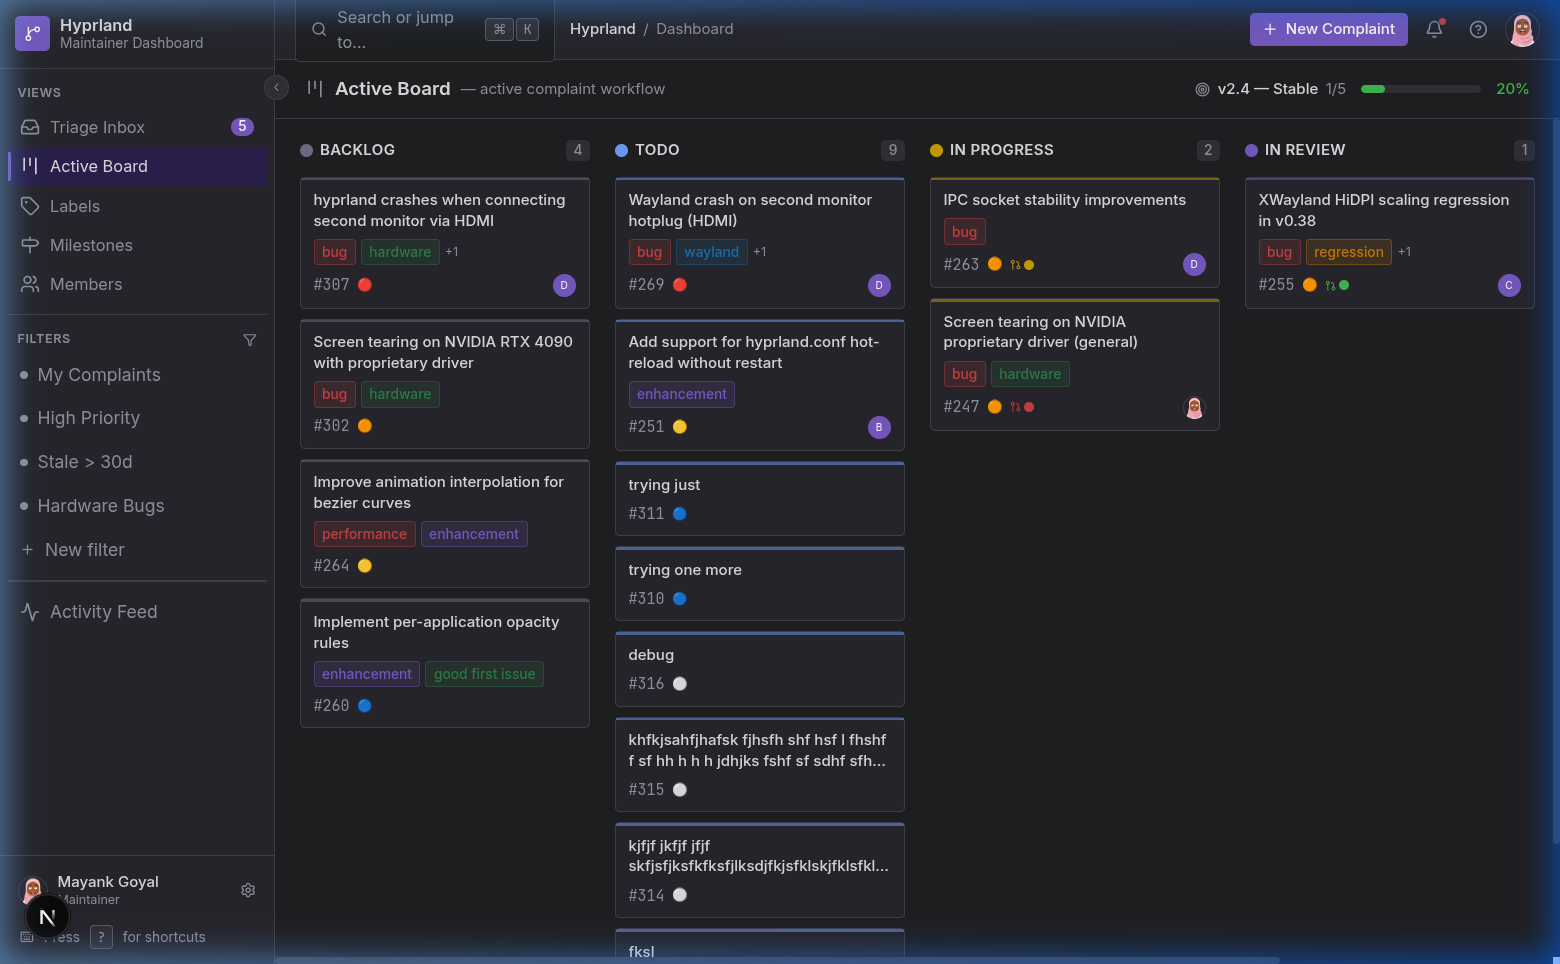
\includegraphics[width=\linewidth]{images/screenshot_kanban.png}
\caption{Kanban Board --- five-column workflow view with drag-and-drop cards}
\label{fig:ss-kanban}
\end{figure}

\vspace{0.5em}
\noindent\textbf{Screenshot 3 --- Issue Drawer}\\[0.5em]
\begin{figure}[H]
\centering
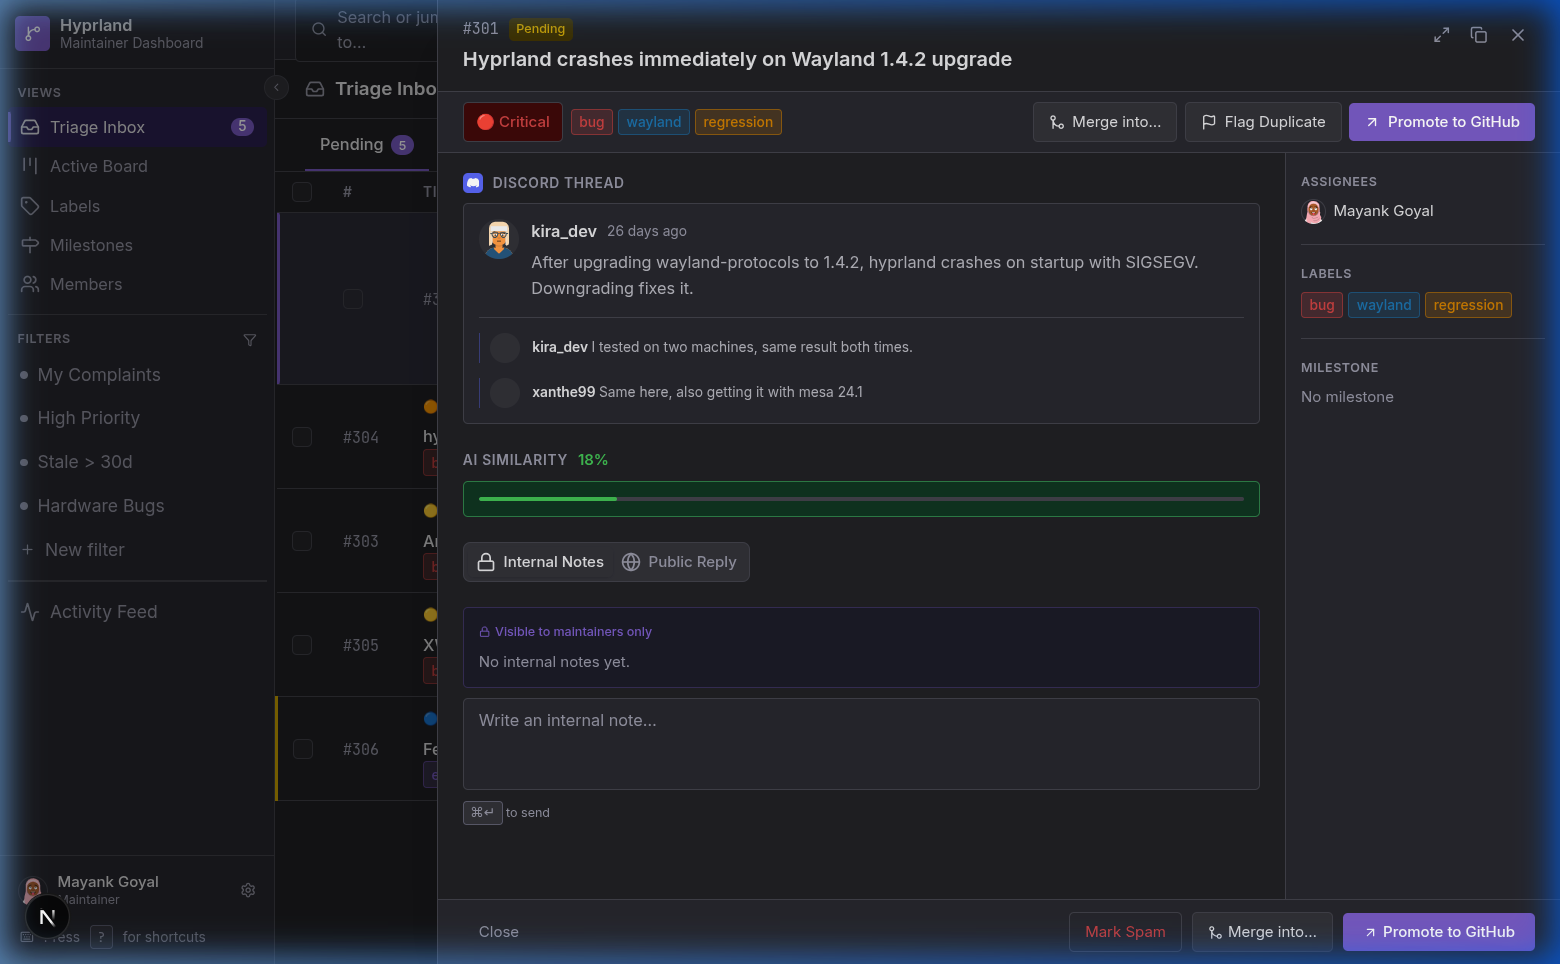
\includegraphics[width=\linewidth]{images/screenshot_drawer.png}
\caption{Issue Drawer --- full issue detail with metadata sidebar and action panel}
\label{fig:ss-drawer}
\end{figure}

\vspace{0.5em}
\noindent\textbf{Screenshot 4 --- Dashboard Overview}\\[0.5em]
\begin{figure}[H]
\centering
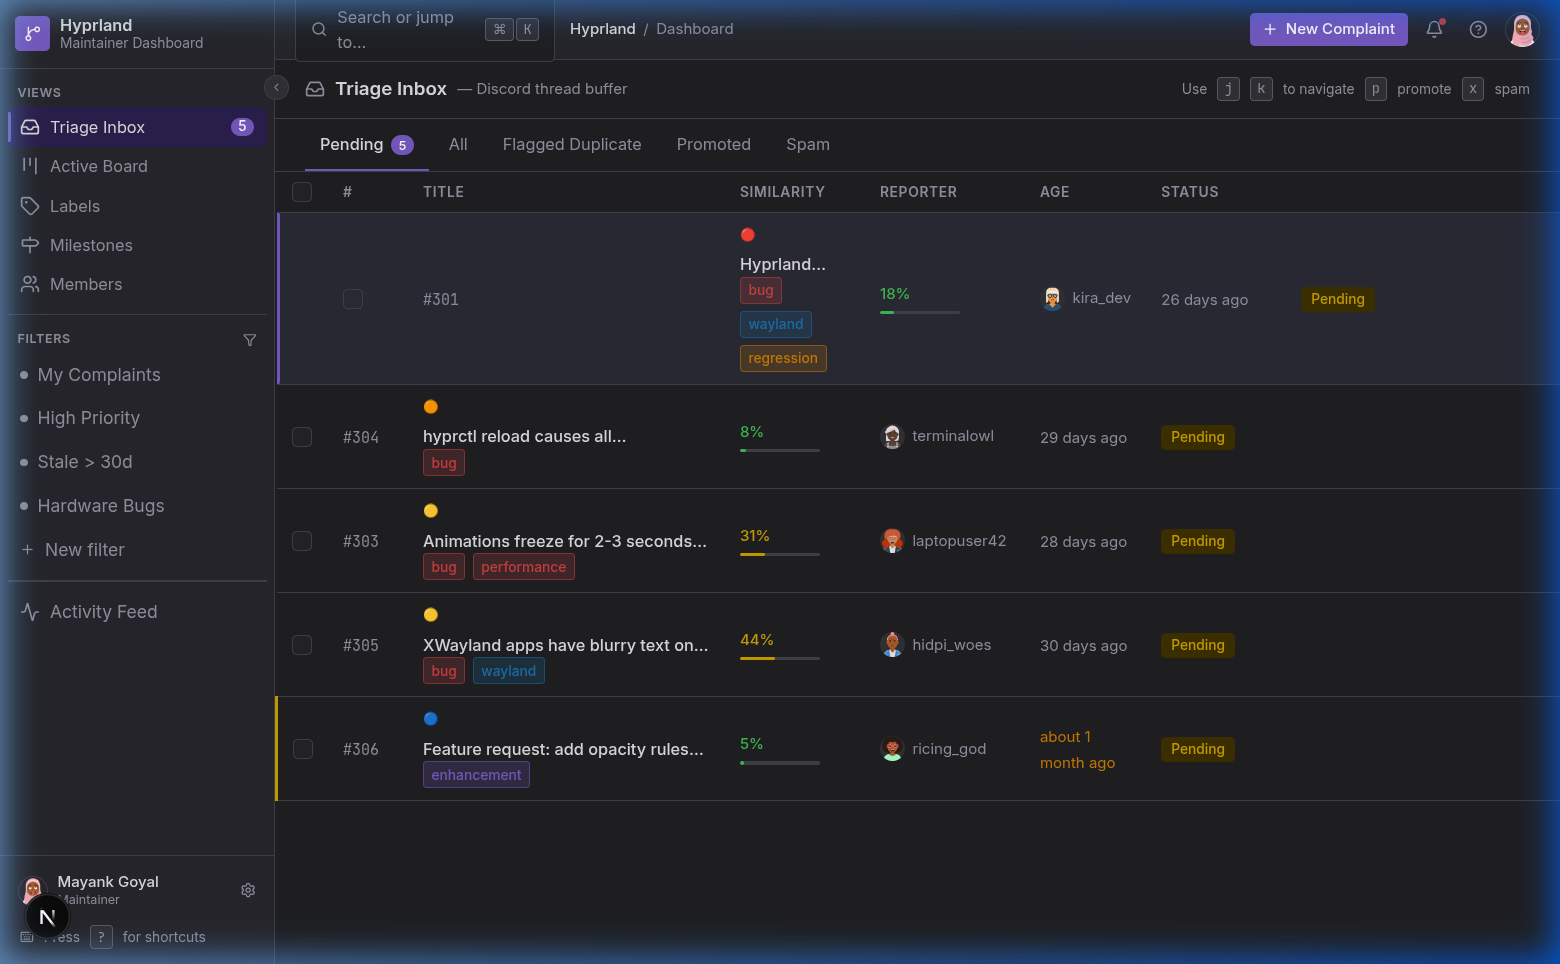
\includegraphics[width=\linewidth]{images/screenshot_dashboard.png}
\caption{Dashboard Overview --- navigation sidebar, triage count badge and main content area}
\label{fig:ss-dashboard}
\end{figure}
%% ============================================================
%%  8.0  USER MANUAL
%% ============================================================
\chapter{User Manual}

\section{Purpose and Scope}

This manual explains how to use the Complaint Management System dashboard
for day-to-day complaint triage and tracking.  The app is designed for
\textbf{maintainers} who need to:
\begin{itemize}
  \item review incoming complaints from Discord,
  \item promote valid complaints into active work,
  \item track active work on a Kanban board,
  \item inspect full issue details in a side drawer,
  \item create new complaints directly.
\end{itemize}

\begin{tcolorbox}[colback=gray!5,colframe=gray!40,title=Scope Clarification]
The UI contains references to Discord and GitHub complaint sources, but direct
external platform integrations require the relevant environment variables to be
configured (\texttt{DISCORD\_BOT\_TOKEN}, \texttt{GITHUB\_TOKEN}).  When these
are absent, the system degrades gracefully: promotion still works locally, but
no external API calls are made.
\end{tcolorbox}

\section{Prerequisites}

\begin{itemize}
  \item Node.js 20 LTS and npm installed.
  \item Docker installed and running (for local PostgreSQL).
\end{itemize}

Start the application:
\begin{lstlisting}[language=bash]
npm install
cp .env.example .env
npm run setup    # starts DB, pushes schema, seeds demo data
npm run dev      # starts Next.js dev server
\end{lstlisting}
Open \texttt{http://localhost:3000}.  The root route redirects automatically
to \texttt{/dashboard/triage}.

\section{Dashboard Layout}

The dashboard is divided into four persistent regions:

\begin{enumerate}
  \item \textbf{Sidebar (left)} --- Main navigation with links to Triage Inbox,
    Active Board, and Settings.  A badge shows the count of pending triage
    items.  The sidebar can be collapsed/expanded.
  \item \textbf{Top Bar (top)} --- Contains the organisation name, a Search /
    command palette trigger, and the ``New Complaint'' button.
  \item \textbf{Main Content (centre)} --- Renders the currently active page
    (Triage, Board, or Settings).
  \item \textbf{Overlay Surfaces} --- Issue Drawer (right panel), Create
    Complaint modal, Command Palette, and the global keyboard handler (invisible
    component).
\end{enumerate}

\section{Triage Inbox}

\textbf{Path:} \texttt{/dashboard/triage}

\subsection{Reading the Table}

Each row in the triage table shows:
\begin{itemize}
  \item \textbf{Checkbox} --- for multi-select / bulk actions.
  \item \textbf{\#} --- sequential complaint number within the organisation.
  \item \textbf{Title} --- complaint title with priority icon and label chips.
    A speech-bubble icon with count shows internal note activity.
  \item \textbf{Similarity} --- AI-computed duplicate score rendered as a
    percentage and colour-coded bar:
    \begin{itemize}
      \item \textcolor{success!80!black}{Green ($< 30\%$)} --- low similarity, likely unique.
      \item \textcolor{warning!80!black}{Amber ($30$--$65\%$)} --- possible duplicate, review recommended.
      \item \textcolor{danger!80!black}{Red ($> 65\%$)} --- high similarity, likely duplicate.
    \end{itemize}
  \item \textbf{Reporter} --- Discord avatar and username.
  \item \textbf{Age} --- relative time since creation; turns amber if stale
    ($> 30$ days).
  \item \textbf{Status} --- coloured badge (Pending, Spam, Promoted, \ldots).
  \item \textbf{Hover Actions} --- Promote ([promote]), Spam ([spam]),
    Open ([open]) icons appear on row hover.
\end{itemize}

\subsection{Filters}

Use the tab bar at the top of the inbox to filter by:
\textbf{Pending} | \textbf{All} | \textbf{Flagged Duplicate} |
\textbf{Promoted} | \textbf{Spam}.

\subsection{Keyboard-Driven Triage}

\begin{longtable}{>{\ttfamily\bfseries}p{2cm} p{10cm}}
\toprule
Key & Action \\
\midrule
\endhead
j & Move cursor down one row. \\
k & Move cursor up one row. \\
Enter & Open Issue Drawer for the focused row. \\
p & Promote the focused complaint to GitHub. \\
x & Mark the focused complaint as spam. \\
e & Mark the focused complaint as done. \\
g t & Navigate to Triage Inbox. \\
g b & Navigate to Active Board. \\
g s & Navigate to Settings. \\
c & Open Create Complaint modal. \\
Ctrl+K & Open Command Palette. \\
Esc & Close open drawer or modal. \\
f & Toggle focus (wide) mode on drawer. \\
\bottomrule
\end{longtable}

\subsection{Bulk Actions}

Select two or more complaints using their checkboxes.  The Bulk Action Bar
appears at the bottom of the screen with:
\begin{itemize}
  \item \textbf{Promote All} --- promotes each selected complaint sequentially.
  \item \textbf{Spam All} --- marks all selected as spam in a single database
    query.
  \item \textbf{Clear Selection} --- deselects all.
\end{itemize}

\section{Active Board}

\textbf{Path:} \texttt{/dashboard/board}

\subsection{Columns}

The board displays five workflow columns for GitHub-source issues:
\begin{enumerate}
  \item \textbf{Backlog} --- promoted but not yet scheduled.
  \item \textbf{Todo} --- queued for implementation.
  \item \textbf{In Progress} --- actively being worked on.
  \item \textbf{In Review} --- pull request open / awaiting review.
  \item \textbf{Done} --- completed.
\end{enumerate}

\subsection{Moving Cards}

Drag a card from one column and drop it onto another.  The UI updates
optimistically and persists the change to the database.  If the server call
fails, the card animates back to its original position and an error toast
appears.

\subsection{Card Information}

Each card shows:
\begin{itemize}
  \item Issue number and truncated title.
  \item Priority dot (colour-coded).
  \item Label chips.
  \item Linked PR number with CI status dot.
  \item Assignee avatar stack.
\end{itemize}

Click any card to open the Issue Drawer for full context.

\subsection{Milestone Progress}

When a milestone is active, the board header shows the milestone title, a
\texttt{closed/total} fraction, a progress bar, and a percentage.

\section{Issue Drawer}

\subsection{Opening and Closing}

\begin{itemize}
  \item \textbf{Open:} click any triage row or board card; press
    \texttt{Enter} on the focused triage row.
  \item \textbf{Close:} press \texttt{Esc}; click the \textbf{X} button;
    click the backdrop; click the footer \textbf{Close} button.
\end{itemize}

\subsection{Drawer Sections}

\begin{longtable}{>{\bfseries}p{4cm} p{9cm}}
\toprule
Section & Content \\
\midrule
\endhead
Header & Issue number, status badge, stale indicator, title, focus/copy/close
  controls. \\
Quick Action Toolbar & Priority chip, label chips, and context-aware CTA
  buttons (Promote / Mark Spam for Discord; View on GitHub / Create Branch for
  GitHub-source). \\
Discord Thread Block & (Discord source only) Original message and replies in
  a threaded layout with Discord-brand colours. \\
Issue Description & (GitHub source) Plain-text description block. \\
AI Similarity Block & Coloured progress bar with score; if
  \texttt{duplicateOfId} is set, shows ``Merge into \#N'' and ``Not a
  duplicate'' buttons. \\
Dual Chat Tabs & \textbf{Internal Notes} tab (purple border, lock icon,
  maintainer-only) and \textbf{Public Reply} tab (green border, globe icon,
  will post to Discord). \\
Metadata Sidebar & Assignees, Labels, Milestone, GitHub issue link, Linked
  PRs with CI dots. \\
Footer & Close, Mark Spam, Merge into (phase-2), Promote to GitHub buttons. \\
\bottomrule
\end{longtable}

\section{Create Complaint}

Open the modal by pressing \texttt{c} or clicking \textbf{New Complaint}
in the top bar.

\begin{longtable}{>{\bfseries}p{3cm} p{9cm}}
\toprule
Field & Details \\
\midrule
\endhead
Title & Required. Maximum 200 words. \\
Description & Optional. Markdown-friendly plain text area. \\
Priority & Drop-down: No Priority, Low, Medium, High, Critical. \\
\bottomrule
\end{longtable}

Submit with \textbf{Create Complaint} button or \texttt{Ctrl+Enter}
(\texttt{Cmd+Enter} on macOS).  The new complaint appears in the Active Board's
\textbf{Todo} column.

\section{Command Palette}

Open with \texttt{Ctrl+K} (or \texttt{Cmd+K} on macOS).

The palette contains three groups:
\begin{itemize}
  \item \textbf{Navigate} --- Go to Triage, Board, Settings.
  \item \textbf{Actions} --- Promote, Mark Spam, Mark Done, Assign, Merge,
    Flag Duplicate.
  \item \textbf{View} --- Toggle Focus Mode.
\end{itemize}

Type to fuzzy-search commands.  Press \texttt{Enter} to execute the highlighted
command.

\section{Troubleshooting}

\begin{longtable}{>{\bfseries}p{5cm} p{8cm}}
\toprule
Symptom & Resolution \\
\midrule
\endhead
App does not load / DB error & Ensure Docker is running. Run
  \texttt{npm run db:up \&\& npm run db:push}. \\
Empty triage or board & Run \texttt{npm run db:seed} to insert demo data. \\
Port 5432 conflict & Stop the conflicting local PostgreSQL service or edit
  \texttt{DATABASE\_URL} in \texttt{.env} and update \texttt{scripts/db-up.sh}. \\
Stale UI after action & Hard-refresh the browser (\texttt{Ctrl+Shift+R}).
  Check the terminal for Prisma/runtime errors. \\
GitHub promotion fails & Verify \texttt{GITHUB\_TOKEN}, \texttt{GITHUB\_OWNER},
  \texttt{GITHUB\_REPO} in \texttt{.env} are correct and token has \texttt{repo}
  scope. \\
Discord reply not sent & Verify \texttt{DISCORD\_BOT\_TOKEN} is set and the
  bot has \textbf{Send Messages} permission in the target forum channel. \\
\bottomrule
\end{longtable}

\section{Daily Workflow Recommendation}

\begin{enumerate}
  \item Start in the \textbf{Triage Inbox} (Pending filter).
  \item Use \texttt{j}/\texttt{k} to navigate; press \texttt{Enter} to open
    the drawer for any complaint that warrants detailed review.
  \item Press \texttt{p} to promote valid complaints; \texttt{x} to spam
    obvious noise.
  \item After triage, switch to the \textbf{Active Board} (\texttt{g b}).
  \item Drag cards across columns to reflect actual work state.
  \item Use the \textbf{Internal Notes} tab in the drawer for team
    communication about sensitive fixes.
  \item Use \textbf{Public Reply} tab to send visible updates back to the
    original Discord reporter.
\end{enumerate}

%% ============================================================
%%  9.0  SUMMARY
%% ============================================================
\chapter{Summary}

\section{Project Achievements}

The Complaint Management System successfully delivers a \textbf{specialised,
keyboard-first triage ecosystem} that addresses the real-world pain-points of
open-source maintainers.  The following capabilities were implemented and are
fully functional in the submitted build:

\begin{longtable}{>{\bfseries}p{4cm} p{9cm}}
\toprule
Feature & Status \\
\midrule
\endhead
Triage Inbox & \textcolor{success!80!black}{\textbf{Implemented}} --- table, filters, cursor, keyboard actions. \\
Promote Pipeline & \textcolor{success!80!black}{\textbf{Implemented}} --- GitHub API, Discord reply, DB update. \\
Spam / Done Actions & \textcolor{success!80!black}{\textbf{Implemented}} --- persist to DB, revalidate. \\
Bulk Promote / Spam & \textcolor{success!80!black}{\textbf{Implemented}} --- multi-select, batch DB update. \\
Kanban Board & \textcolor{success!80!black}{\textbf{Implemented}} --- DnD, optimistic update, 5 columns. \\
Issue Drawer & \textcolor{success!80!black}{\textbf{Implemented}} --- animated, fetch, full context. \\
AI Similarity Display & \textcolor{success!80!black}{\textbf{Implemented}} --- score bar, colour coding, duplicate hint. \\
Create Complaint & \textcolor{success!80!black}{\textbf{Implemented}} --- modal, validation, DB persist. \\
Command Palette & \textcolor{success!80!black}{\textbf{Implemented}} --- cmdk, grouped commands. \\
Keyboard Shortcuts & \textcolor{success!80!black}{\textbf{Implemented}} --- tinykeys, j/k/p/x/e/f/g-seq. \\
Discord Chat Integration & \textcolor{warning!80!black}{\textbf{Phase 2}} --- UI renders thread; live bot requires token. \\
Note Persistence & \textcolor{warning!80!black}{\textbf{Phase 2}} --- UI shows toast; actual save deferred. \\
Merge / Flag Duplicate & \textcolor{warning!80!black}{\textbf{Phase 2}} --- buttons present; action shows toast. \\
Assign to Me & \textcolor{warning!80!black}{\textbf{Phase 2}} --- keyboard event fires; DB write deferred. \\
Public Read-Only Mirror & \textcolor{warning!80!black}{\textbf{Phase 2}} --- architecture designed, not deployed. \\
\bottomrule
\end{longtable}

\section{Key Design Decisions}

\begin{enumerate}
  \item \textbf{Server Actions over Traditional API Routes} --- Using Next.js
    Server Actions for all mutations eliminates the need for a separate
    REST API layer for writes, keeping secrets server-side automatically and
    reducing boilerplate significantly.
  \item \textbf{Zustand for Local UI State} --- The drawer open/close state,
    bulk selection set, and triage cursor index are lightweight client-only
    concerns.  Zustand provides these without the overhead of a global server
    state manager.
  \item \textbf{Prisma Schema-as-Truth} --- Using \texttt{prisma db push} in
    development means the schema file is the single source of truth for the
    database structure, eliminating schema drift.
  \item \textbf{Optimistic UI for Kanban} --- The board update applies
    immediately on drag-end, making the experience feel instantaneous.
    Rollback on failure ensures consistency.
  \item \textbf{Graceful Integration Degradation} --- Both GitHub and Discord
    integrations are wrapped in feature-flag checks
    (\texttt{isGitHubIntegrationEnabled()},
    \texttt{isDiscordBotEnabled()}).  This means the application is
    fully functional as a standalone tool without any external accounts.
\end{enumerate}

\section{Lessons Learned}

\begin{itemize}
  \item React Server Components require careful boundary placement: data
    fetching belongs in RSCs, event handlers and state belong in Client
    Components marked \texttt{"use client"}.
  \item The \texttt{@dnd-kit} library required careful configuration of
    collision detection (\texttt{closestCorners}) to correctly identify the
    target column when dragging between columns of different sizes.
  \item Discord's \texttt{discordReplies} JSON field (stored as
    \texttt{Json?}) provides flexibility but requires defensive null-checking
    throughout the UI layer.
  \item The \texttt{revalidatePath} calls after Server Actions are critical for
    keeping server-rendered pages in sync after mutations; missing a call
    results in stale data being displayed.
\end{itemize}

\section{Future Work}

\begin{enumerate}
  \item Implement full \textbf{NextAuth.js} authentication with GitHub OAuth
    and organisation membership verification.
  \item Build the \textbf{AI embedding pipeline} (e.g., using
    \texttt{pgvector} + OpenAI embeddings) to compute and store
    \texttt{similarityScore} in real time on issue ingest.
  \item Deploy the \textbf{public read-only mirror} as a statically generated
    Next.js site with ISR (Incremental Static Regeneration).
  \item Implement \textbf{note persistence} (complete the \texttt{createNote}
    server action wired to the textarea submit).
  \item Add \textbf{label and assignee management} UI in the Settings page.
  \item Implement the \textbf{merge-duplicate} workflow in full, including
    status update, cross-linking, and Discord notification.
  \item Add \textbf{webhook ingestion} endpoint to receive Discord Forum events
    automatically rather than requiring manual data import.
\end{enumerate}

\end{document}
